\documentclass{article}
\usepackage{ctex}
\usepackage{geometry}
\geometry{a4paper, scale=0.8}
\usepackage{graphicx}
\usepackage{float}
\usepackage{enumitem}
\usepackage{amsmath}
\usepackage{amssymb}
\usepackage{hyperref}
\hypersetup{
    hypertex=true,
    colorlinks=true,
    linkcolor=black,
    anchorcolor=black,
    citecolor=black
}
\usepackage{fontspec}
\newfontfamily\jetbrains{JetBrains Mono}
\usepackage{listings}
\usepackage{color}
\lstset{
    breaklines,                                 % 自动将长的代码行换行排版
    extendedchars=false,                        % 解决代码跨页时,章节标题,页眉等汉字不显示的问题
    backgroundcolor=\color[rgb]{0.96,0.96,0.96},% 背景颜色
    keywordstyle=\color{blue}\bfseries,         % 关键字颜色
    identifierstyle=\color{black},              % 普通标识符颜色
    commentstyle=\color[rgb]{0,0.6,0},          % 注释颜色
    stringstyle=\color[rgb]{0.58,0,0.82},       % 字符串颜色
    showstringspaces=false,                     % 不显示字符串内的空格
    numbers=left,                               % 显示行号
    numberstyle=\tiny\jetbrains,                    % 设置数字字体
    basicstyle=\small\jetbrains,                    % 设置基本字体
    captionpos=t,                               % title在上方(在bottom即为b)
    frame=single,                               % 设置代码框形式
    rulecolor=\color[rgb]{0.8,0.8,0.8},         % 设置代码框颜色
}
\usepackage{subfigure}


\title{数据库Lab 03实验报告 \\ \small{银行业务管理系统系统设计与实现报告}}
\author{PB19071405 \ 王昊元}
\date{2022 年 06 月 10 日}

\begin{document}
    \maketitle
    \thispagestyle{empty}

    \newpage
    \tableofcontents
    \thispagestyle{empty}

    \newpage
    \setcounter{page}{1}

    \section{概述}
    \subsection{系统目标}
    开发一个银行业务管理系统,该系统基于MySQL,使用Python进行后端开发,使用HTML+CSS+JavaScript进行前端开发,
    主要以谷歌浏览器作为目标浏览器,实现客户、账户、贷款、业务以及其它方面的去求。
    \subsection{需求说明}
    银行有多个支行。各个支行位于某个城市,每个支行有唯一的名字。银行要监控每个支行的资产。

    银行的客户通过其身份证号来标识。银行存储每个客户的姓名、联系电话以及家庭住址。
    为了安全起见,银行还要求客户提供一位联系人的信息,包括联系人姓名、手机号、Email以及与客户的关系。
    客户可以有帐户,并且可以贷款。客户可能和某个银行员工发生联系,该员工是此客户的贷款负责人或银行帐户负责人。
    
    银行员工也通过身份证号来标识。员工分为部门经理和普通员工,每个部门经理都负责领导其所在部门的员工,并且每个员工只允许在一个部门内工作。
    每个支行的管理机构存储每个员工的姓名、电话号码、家庭地址、所在的部门号、部门名称、部门类型及部门经理的身份证号。
    银行还需知道每个员工开始工作的日期,由此日期可以推知员工的雇佣期。
    
    银行提供两类帐户——储蓄帐户和支票帐户。帐户可以由多个客户所共有,一个客户也可开设多个账户,但在一个支行内最多只能开设一个储蓄账户和一个支票账户。
    每个帐户被赋以唯一的帐户号。银行记录每个帐户的余额、开户日期、开户的支行名以及每个帐户所有者访问该帐户的最近日期。
    另外,每个储蓄帐户有利率和货币类型,且每个支票帐户有透支额。每笔贷款由某个分支机构发放,能被一个或多个客户所共有。
    每笔贷款用唯一的贷款号标识。银行需要知道每笔贷款所贷金额以及逐次支付的情况(银行将贷款分几次付给客户)。
    虽然贷款号不能唯一标识银行所有为贷款所付的款项,但可以唯一标识为某贷款所付的款项。对每次的付款需要记录日期和金额。

    主要功能需求:
    \begin{itemize}
        \item 客户管理:提供客户所有信息的增、删、改、查功能;如果客户存在着关联账户或者贷款记录,则不允许删除
        \item 账户管理:提供账户开户、销户、修改、查询功能,包括储蓄账户和支票账户;账户号不允许修改
        \item 贷款管理:提供贷款信息的增、删、查功能,提供贷款发放功能;贷款信息一旦添加成功后不允许修改;要求能查询每笔贷款的当前状态(未开始发放、发放中、已全部发放);处于发放中状态的贷款记录不允许删除
        \item 业务统计:按业务分类(储蓄、贷款)和时间(月、季、年)统计各个支行的业务总金额和用户数,统计的结果以表格形式展示
    \end{itemize}
    \subsection{本报告的主要贡献}
    \begin{itemize}
        \item 建立数据库结构模型
        \item 展示数据库各个模块的实现
        \item 对各个模块进行测试评估
        \item 进行实验总结
    \end{itemize}
    \section{总体设计}
    \subsection{系统模块结构}
    \begin{figure}[H]
        \centering
        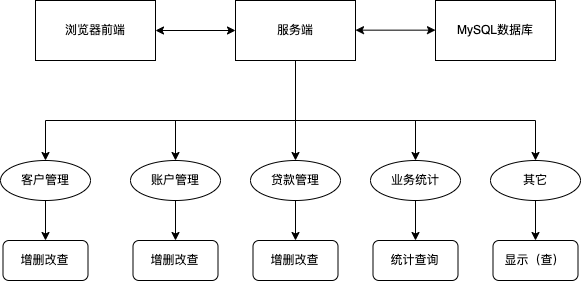
\includegraphics[width=0.8\textwidth]{./fig/system_module.png}
        \caption[system_module]{系统模块结构示意图}
    \end{figure}
    \begin{itemize}
        \item 实现采用浏览器/服务器架构,基于MySQL数据库,使用Python进行后端开发,
        使用HTML+CS+JavaScript进行前端开发
        \item 主要实现客户管理(增删改查)、账户管理(增删改查)、贷款管理(增删改查)、业务统计(查询并统计)及其它一些信息的查询功能
        \item 尝试开发用户登陆模块,但由于能力有限,功能还处于使用数据库记录注册账户信息阶段,并未涉及任何权限相关
    \end{itemize}
    \subsection{系统工作流程}
    \begin{figure}[H]
        \centering
        
\includegraphics[width=0.8\textwidth]{./fig/working_pipeline.png}
        \caption[working_pipeline]{系统工作流程示意图}
    \end{figure}
    \begin{itemize}
        \item 增加
        \begin{itemize}
            \item 用户在输入框中输入信息(前端进行一些检查,例如必填项)
            \item 用户提交信息后,后端根据内容生成MySQL语句
            \item 对数据库执行MySQL语句,将数据写入数据库
            \item 后端对数据库的执行情况进行检查,并将结果返回用户
        \end{itemize}
        \item 删除
        \begin{itemize}
            \item 用户点击要删除的信息所对应的删除按钮
            \item 前端将对应要删除的信息传输给后端
            \item 后端根据信息生成MySQL语句并执行
            \item 根据数据库的执行情况进行检查,并将结果返回用户
        \end{itemize}
        \item 修改
        \begin{itemize}
            \item 用户点击要修改的信息对应的修改按钮
            \item 用户填写新的信息
            \item 前端将要修改的信息和修改后的信息传输给后端
            \item 后端根据信息生成MySQL语句并执行
            \item 根据数据库的执行情况进行检查,并将结果返回用户
        \end{itemize}
        \item 查询
        \begin{itemize}
            \item 用户在输入框中输入查询信息
            \item 用户提交查询信息
            \item 前端将查询信息传输给后端
            \item 后端根据信息生成MySQL语句并执行
            \item 对查询结果进行检查,并将结果返回用户
        \end{itemize}
    \end{itemize}
    \subsection{数据库设计}
    \begin{figure}[H]
        \centering
        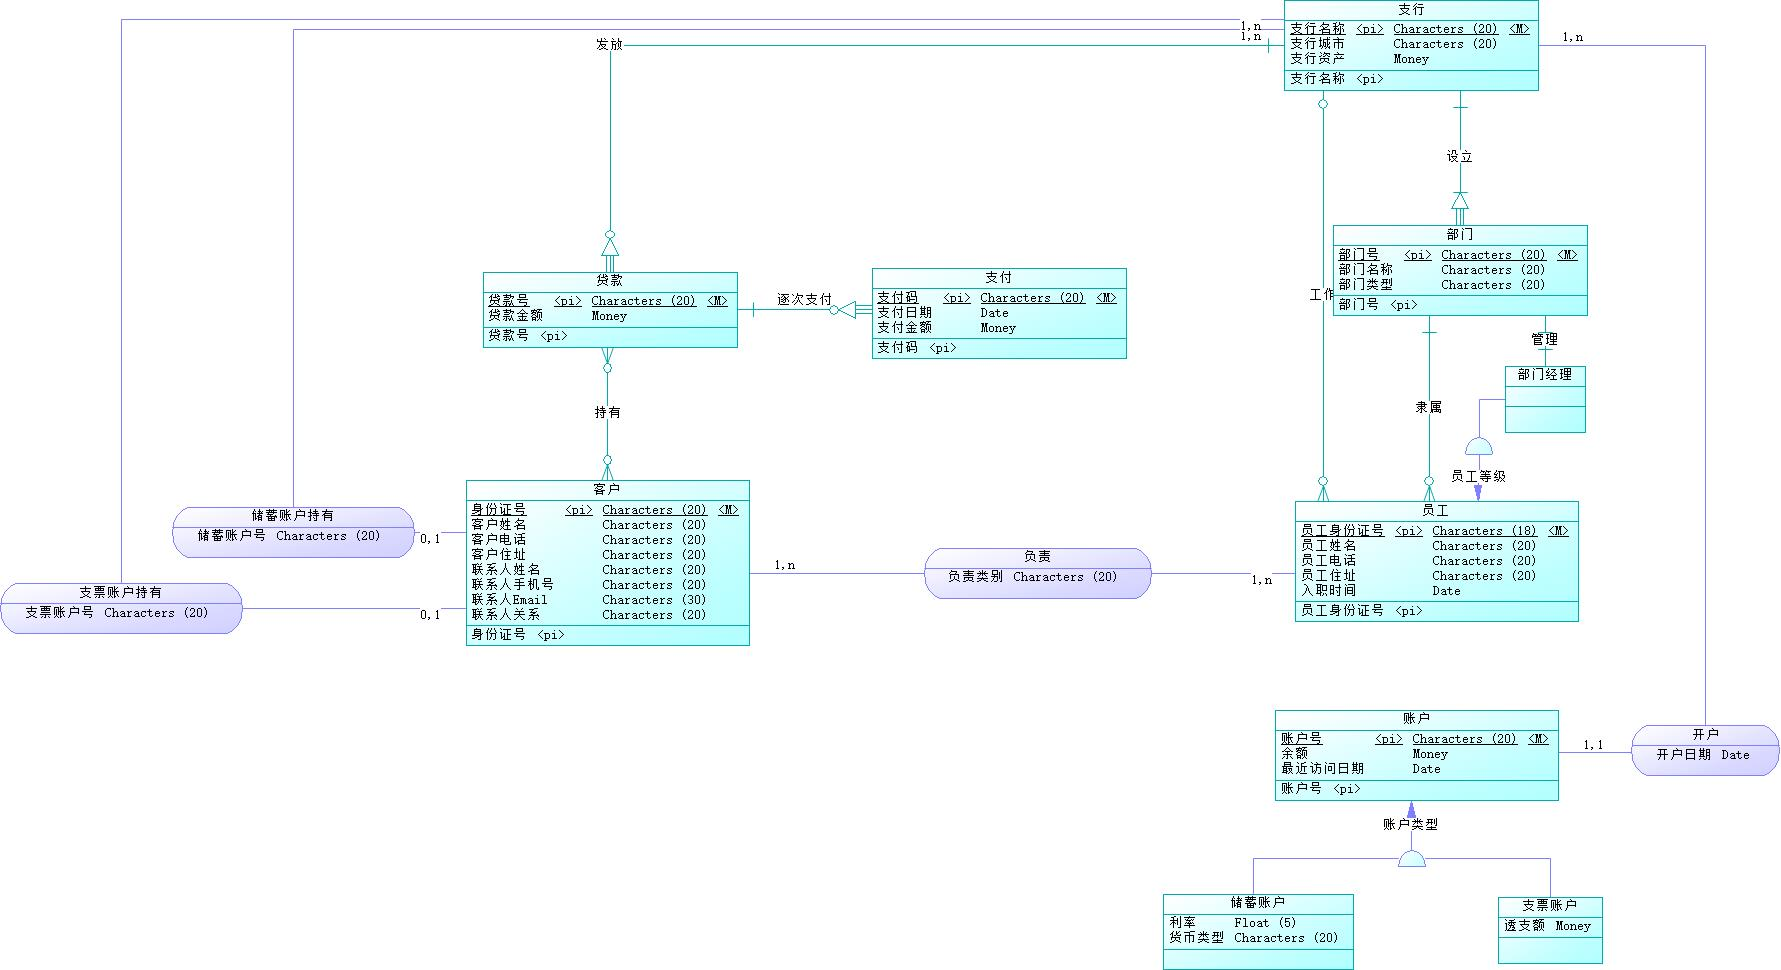
\includegraphics[width=0.8\textwidth]{./fig/cdm.jpg}
        \caption[er]{数据库设计ER图}
    \end{figure}
    \begin{lstlisting}[language=sql]
# 账户(账户号,支行名,余额,开户日期)
create table Account
(
    Account_ID varchar(50) not null,
    Bank_Name varchar(50) not null,
    Balance float(15),
    Opening_Date date,
    primary key (Account_ID)
);

# 支付(用户号,贷款号,支付号,支付金额,支付日期)
create table Pay
(
    Client_ID varchar(50) not null,
    Loan_ID varchar(50),
    Pay_ID varchar(50) not null,
    Pay_Amount float(15),
    Pay_Date date,
    primary key (Client_ID, Loan_ID, Pay_ID)
);

# 支行(支行,城市,资产)
create table Bank(
    Bank_Name varchar(50) not null,
    City varchar(50) not null,
    Assets float(15) not null,
    primary key (Bank_Name)
);

# 支票账户(账户号,透支额)
create table Cheque_Account
(
    Account_ID varchar(50) not null,
    Overdraft float(15),
    primary key (Account_ID)
);

# 客户(客户号,客户名,客户电话,客户地址)
create table Client
(
    Client_ID varchar(50) not null,
    Client_Name varchar(50) not null,
    Client_Tel varchar(50),
    Client_Address varchar(50),
    primary key (Client_ID)
);

# 联系人(客户号,联系人名,联系人邮箱,联系人电话,联系人和客户的关系)
create table Contact
(
    Client_ID varchar(50) not null,
    Contact_Name varchar(50) not null,
    Contact_Email varchar(50),
    Contact_Tel varchar(50),
    Relation varchar(50),
    primary key (Client_ID, Contact_Name)
);

# 部门(部门号,部门名,部门类型,经理身份证号)
create table Department
(
    Department_ID varchar(50) not null,
    Department_Name varchar(50) not null,
    Department_Type varchar(50),
    Manager_ID varchar(50),
    primary key (Department_ID)
);

# 员工(员工号,员工名,支行名,部门名,员工电话,员工地址,入职日期)
create table Employee
(
    Employee_ID varchar(50) not null,
    Employee_Name varchar(50) not null,
    Bank_Name varchar(50) not null,
    Department_ID varchar(50),
    Employee_Tel varchar(50),
    Employee_Address varchar(50),
    Work_Date date,
    primary key (Employee_ID)
);

# 贷款(贷款号,支行名,贷款总额,状态,已支付贷款)
create table Loan
(
    Loan_ID varchar(50) not null,
    Bank_Name varchar(50) not null,
    Loan_Amount float(15) not null,
    Loan_Status int default 0 not null,
    Pay_already float(15) not null,
    Opening_Date date,
    primary key (Loan_ID)
);

# 持有(客户号,最近访问日期,账户名)
create table Own
(
    Client_ID varchar(50) not null,
    Visited_Date date,
    Account_ID varchar(50),
    primary key (Client_ID, Account_ID)
);

# 开户约束(客户号,银行名,账户类型)
create table Checking
(
    Client_ID varchar(50) not null,
    Bank_Name varchar(50) not null,
    Account_Type int not null,
    primary key (Client_ID, Bank_Name, Account_Type)
);

# 储蓄账户(账户号,利率,货币类型)
create table Saving_Account
(
    Account_ID varchar(50) not null,
    Interest_Rate float(15),
    Currency_Type varchar(50),
    primary key (Account_ID)
);

# 服务(客户号,员工号,服务类型:该员工是此客户的贷款负责人或银行帐户负责人)
create table Service
(
    Client_ID varchar(50) not null,
    Employee_ID varchar(50) not null,
    Service_Type varchar(50),
    primary key (Client_ID, Employee_ID)
);

alter table Account add constraint FK_Open foreign key (Bank_Name)
        references Bank (Bank_Name) on delete restrict on update restrict;

alter table Pay add constraint FK_Apply foreign key (Client_ID)
        references Client (Client_ID) on delete restrict on update restrict;

alter table Cheque_Account add constraint FK_Account_Type foreign key (Account_ID)
        references Account (Account_ID) on delete restrict on update restrict;

alter table Contact add constraint FK_Have foreign key (Client_ID)
        references Client (Client_ID) on delete restrict on update restrict;

alter table Employee add constraint FK_Belong_To foreign key (Department_ID)
        references Department (Department_ID) on delete restrict on update restrict;

alter table Employee add constraint FK_Employ foreign key (Bank_Name)
        references Bank (Bank_Name) on delete restrict on update restrict;

alter table Loan add constraint FK_Make_Loan foreign key (Bank_Name)
        references Bank (Bank_Name) on delete restrict on update restrict;

alter table Own add constraint FK_Own1 foreign key (Client_ID)
        references Client (Client_ID) on delete restrict on update restrict;

alter table Own add constraint FK_Own2 foreign key (Account_ID)
        references Account (Account_ID) on delete restrict on update restrict;

alter table Saving_Account add constraint FK_Account_Type2 foreign key (Account_ID)
        references Account (Account_ID) on delete restrict on update restrict;

alter table Service add constraint FK_Service foreign key (Client_ID)
        references Client (Client_ID) on delete restrict on update restrict;

alter table Service add constraint FK_Service2 foreign key (Employee_ID)
        references Employee (Employee_ID) on delete restrict on update restrict;

alter table Checking add constraint FK_Checking1 foreign key (Client_ID)
        references Client (Client_ID) on delete restrict on update restrict;

alter table Checking add constraint FK_Checking2 foreign key (Bank_Name)
        references Bank (Bank_Name) on delete restrict on update restrict;
    \end{lstlisting}
    \section{详细设计(部分)}
    因为个人设计得较为简单,输入基本都是必要的信息,输出基本都是响应的页面,程序流程图也较为简单,
    所以就不详细展开每个模块单独讲了。
    在这里对几个个人认为需要说明的点进行简单说明
    \begin{itemize}
        \item 每个部分要尽力处理可能出现的能想到的异常情况,其余的异常情况要显示在log中。
        例如:删除一个有账户的客户是非法的、删除一个未结算清的贷款是非法的、贷款支付金额是不能大于贷款金额的、金额是不能为负的等等等等。
        \item 用户提供信息有误的情况/用户操作非法的情况,需要提示用户,例如:
        \begin{figure}[H]
            \centering
            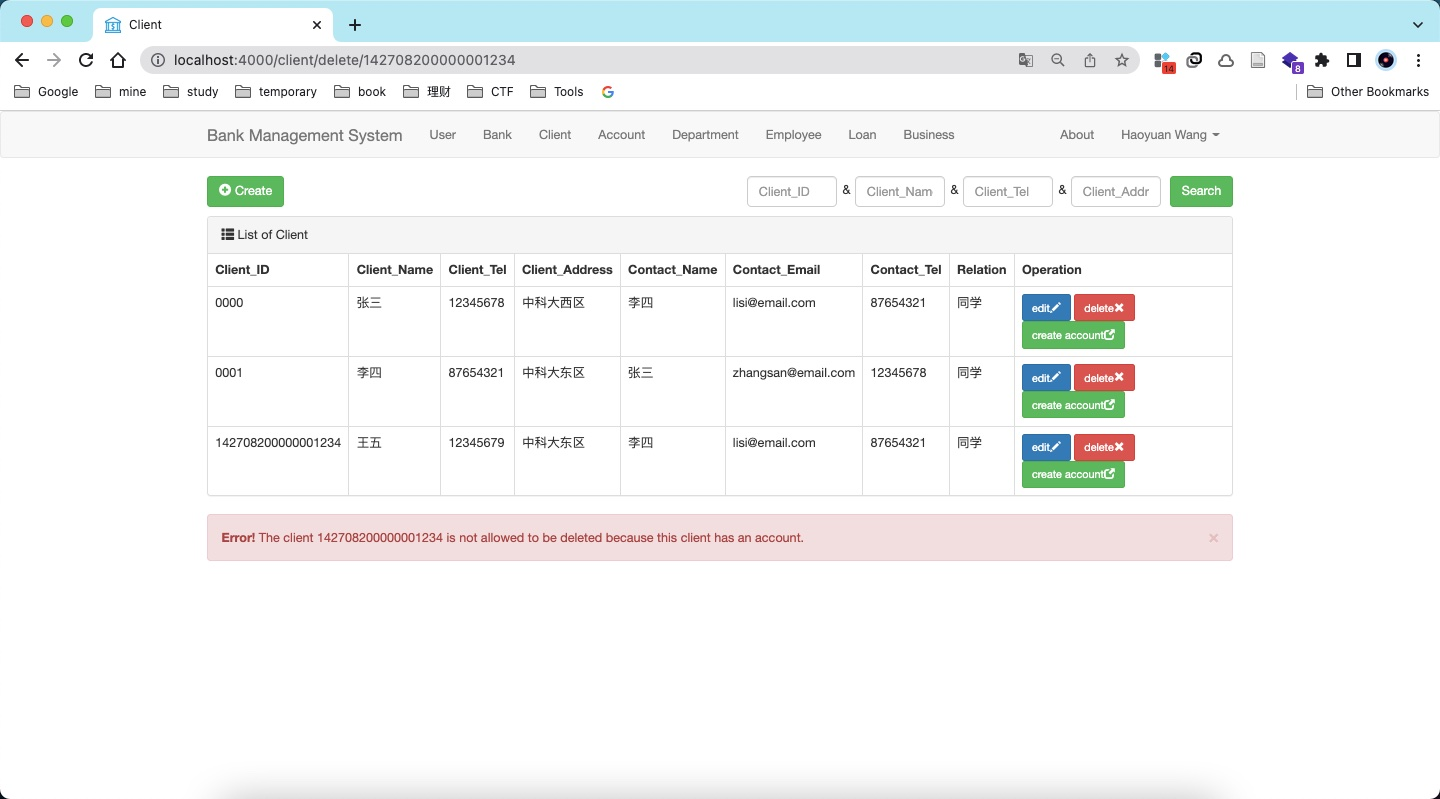
\includegraphics[width=0.7\textwidth]{./fig/delete_account_error.jpg}
            \caption{异常情况提示示例}
        \end{figure}
        \item 对于信息的正确性和合理性,前端和后端都应尽力去检查(这点我做的可能不够完美,但我尽力地去做了)
    \end{itemize}
    \section{实现与测试}
    \subsection{实现结果}
    \begin{figure}[H]
        \centering
        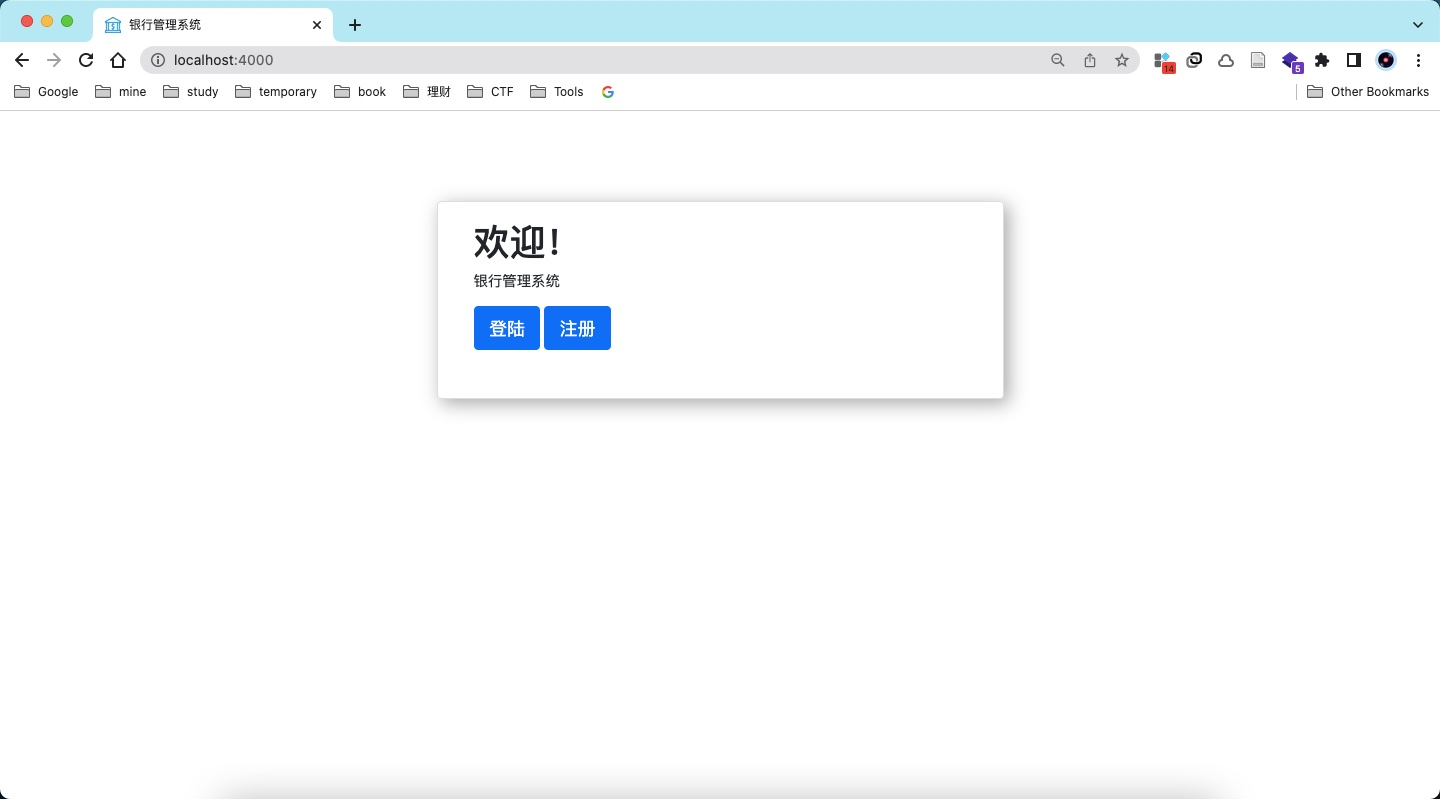
\includegraphics[width=0.8\textwidth]{./fig/index.jpg}
        \caption[index]{首页}
    \end{figure}
    \begin{figure}[H]
        \centering
        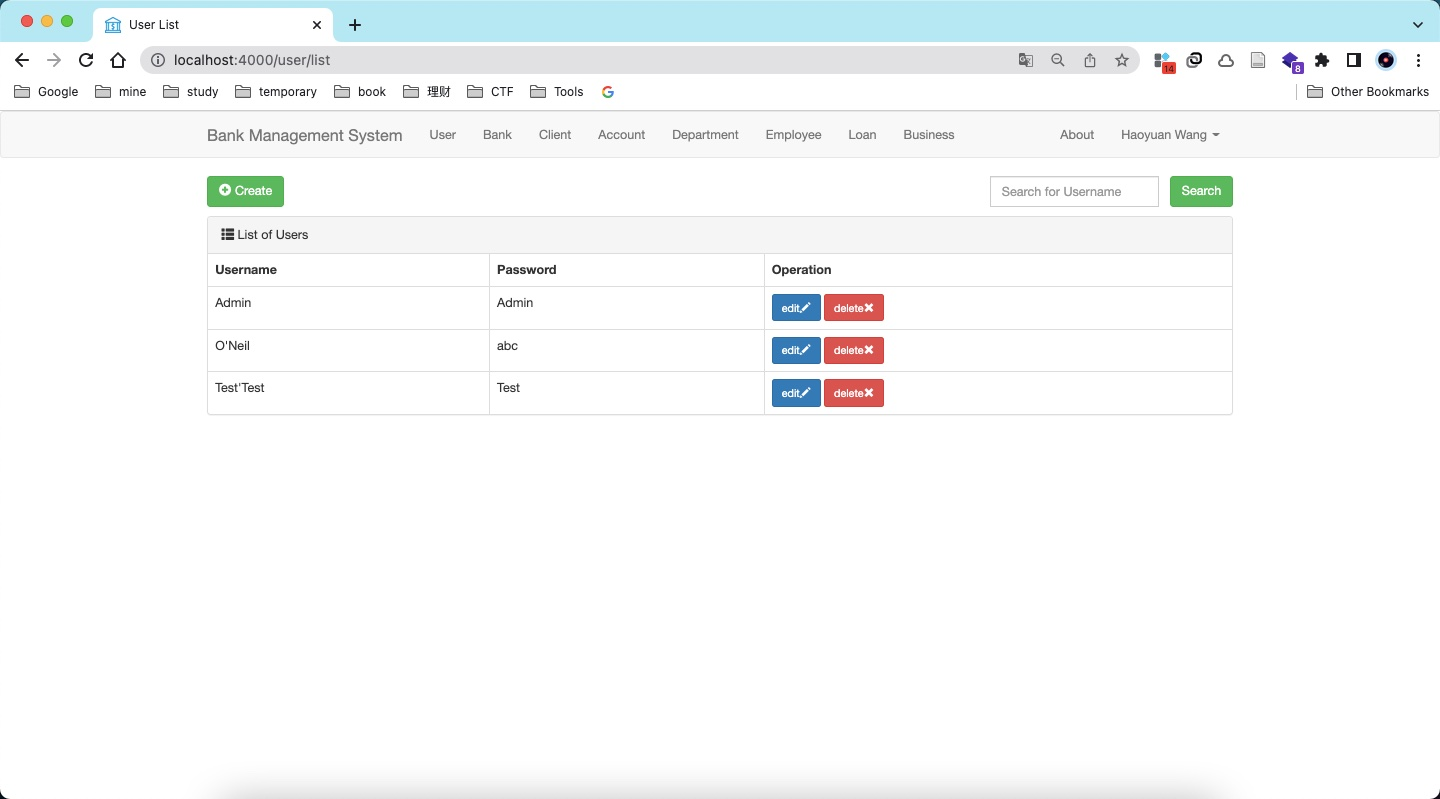
\includegraphics[width=0.8\textwidth]{./fig/user_list.jpg}
        \caption[user_list]{系统用户列表}
    \end{figure}
    \begin{figure}[H]
        \centering
        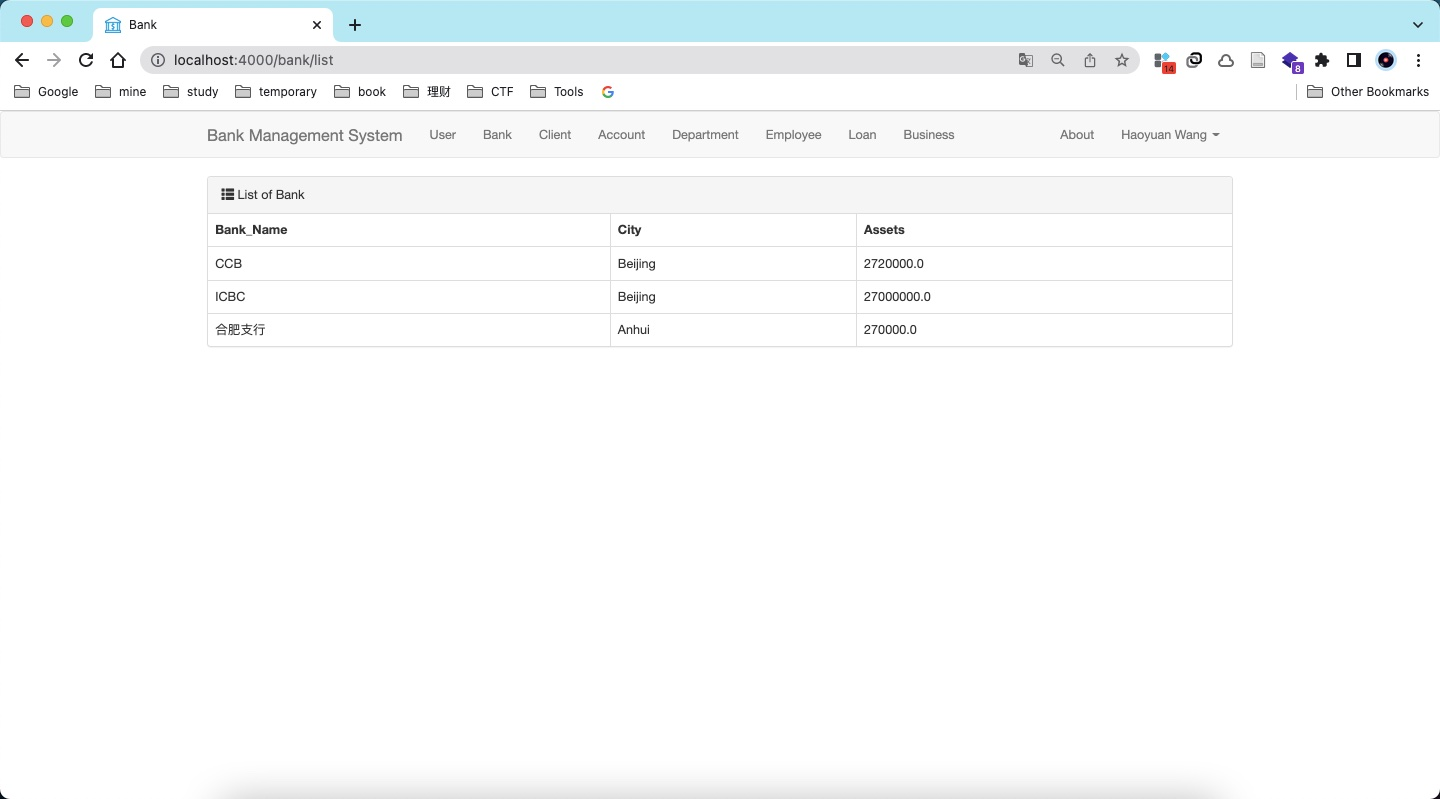
\includegraphics[width=0.8\textwidth]{./fig/bank_list.jpg}
        \caption[bank_list]{支行列表}
    \end{figure}
    \begin{figure}[H]
        \centering
        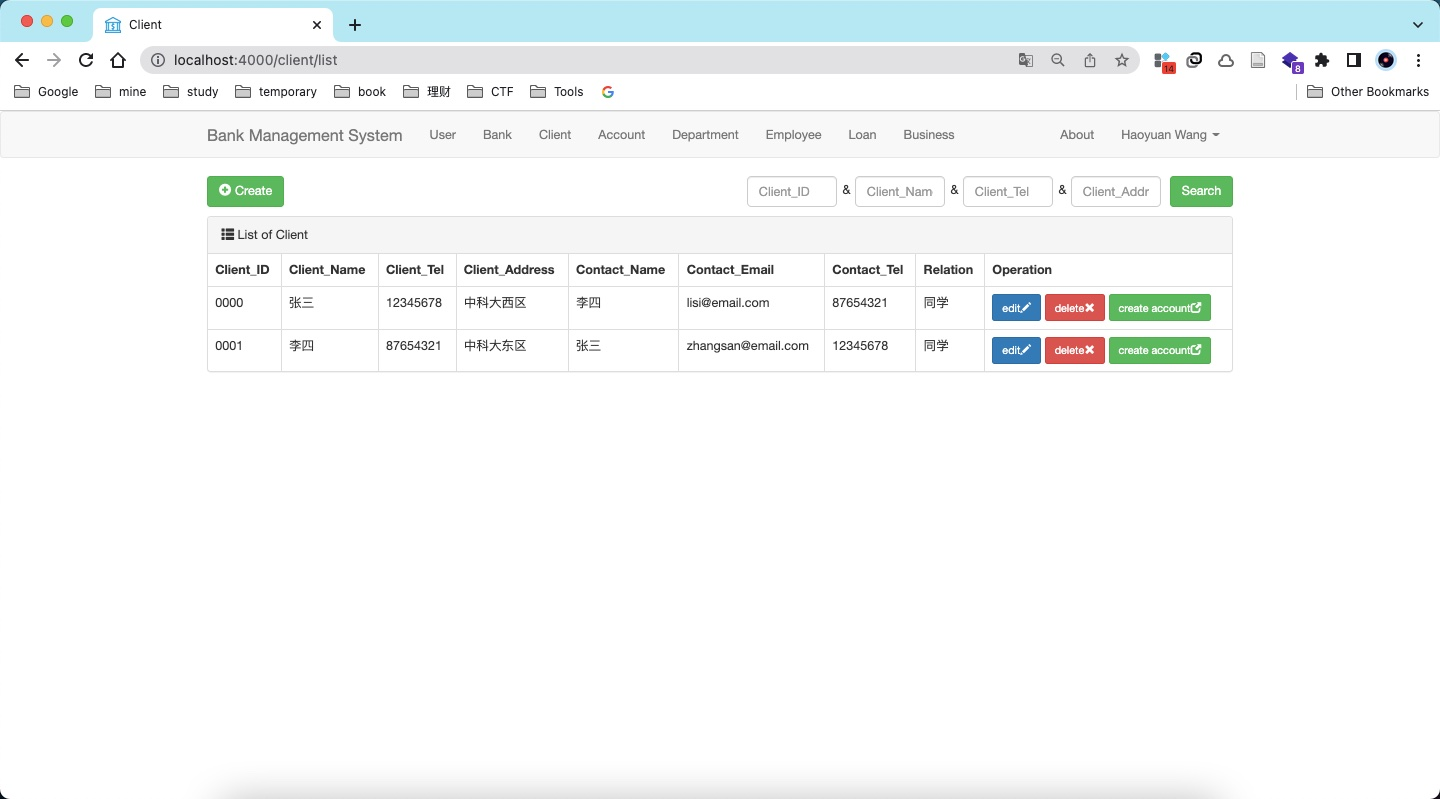
\includegraphics[width=0.8\textwidth]{./fig/client_list.jpg}
        \caption[client_list]{客户列表}
    \end{figure}
    \begin{figure}[H]
        \centering
        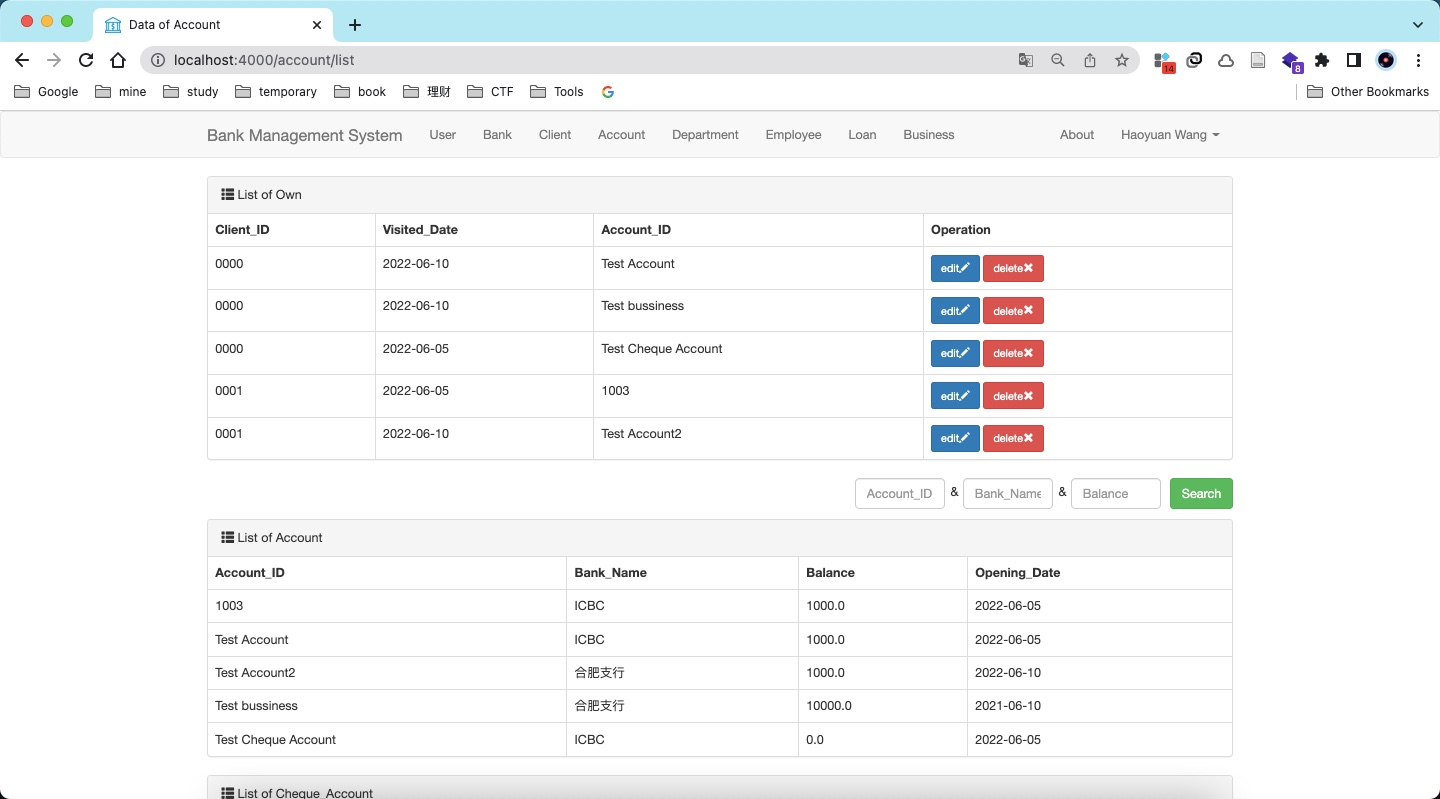
\includegraphics[width=0.8\textwidth]{./fig/account_list.jpg}
        \caption[account_list]{账户列表}
    \end{figure}
    \begin{figure}[H]
        \centering
        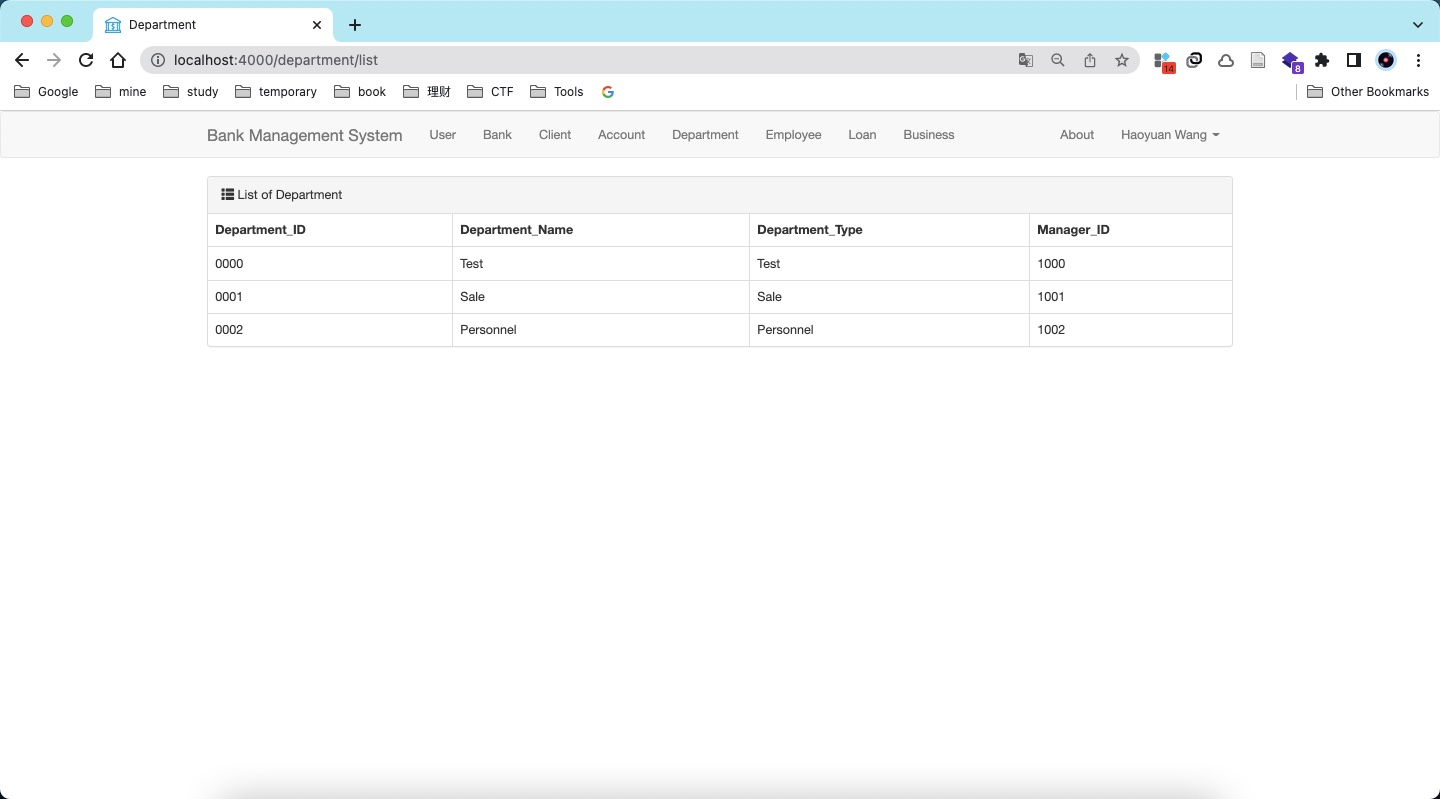
\includegraphics[width=0.8\textwidth]{./fig/department_list.jpg}
        \caption[department_list]{部门列表}
    \end{figure}
    \begin{figure}[H]
        \centering
        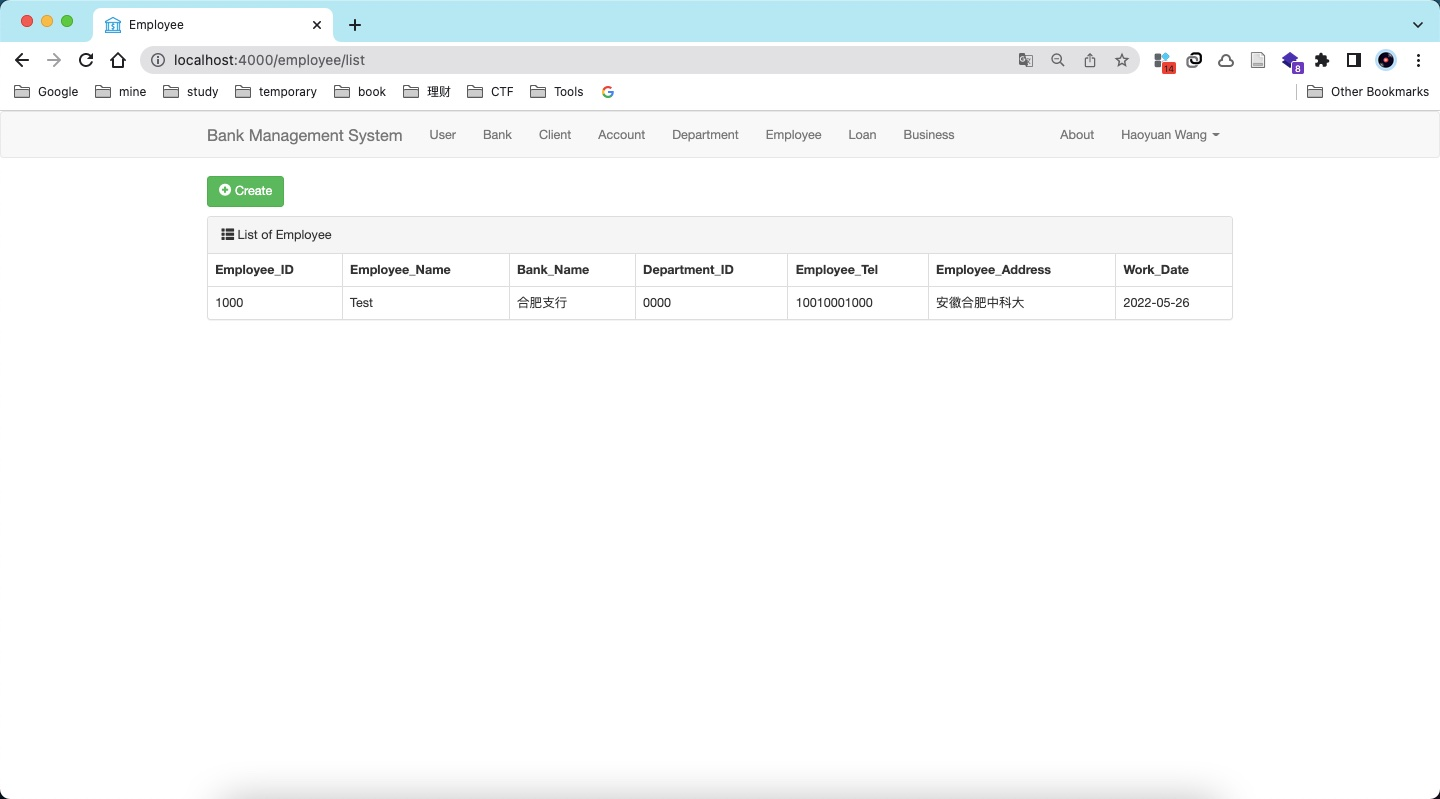
\includegraphics[width=0.8\textwidth]{./fig/employee_list.jpg}
        \caption[employee_list]{职员列表}
    \end{figure}
    \begin{figure}[H]
        \centering
        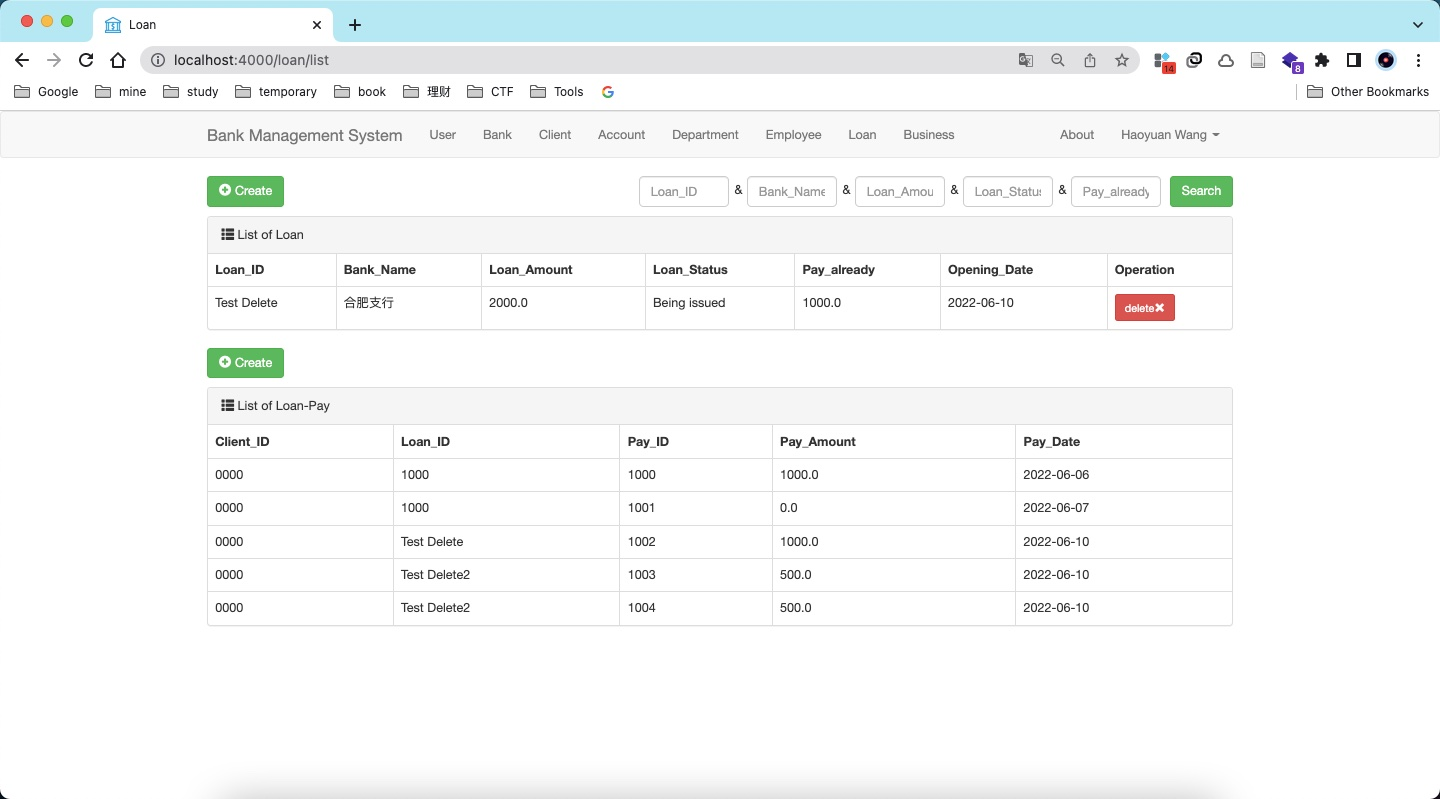
\includegraphics[width=0.8\textwidth]{./fig/loan_list.jpg}
        \caption[loan_list]{贷款列表}
    \end{figure}
    \begin{figure}[H]
        \centering
        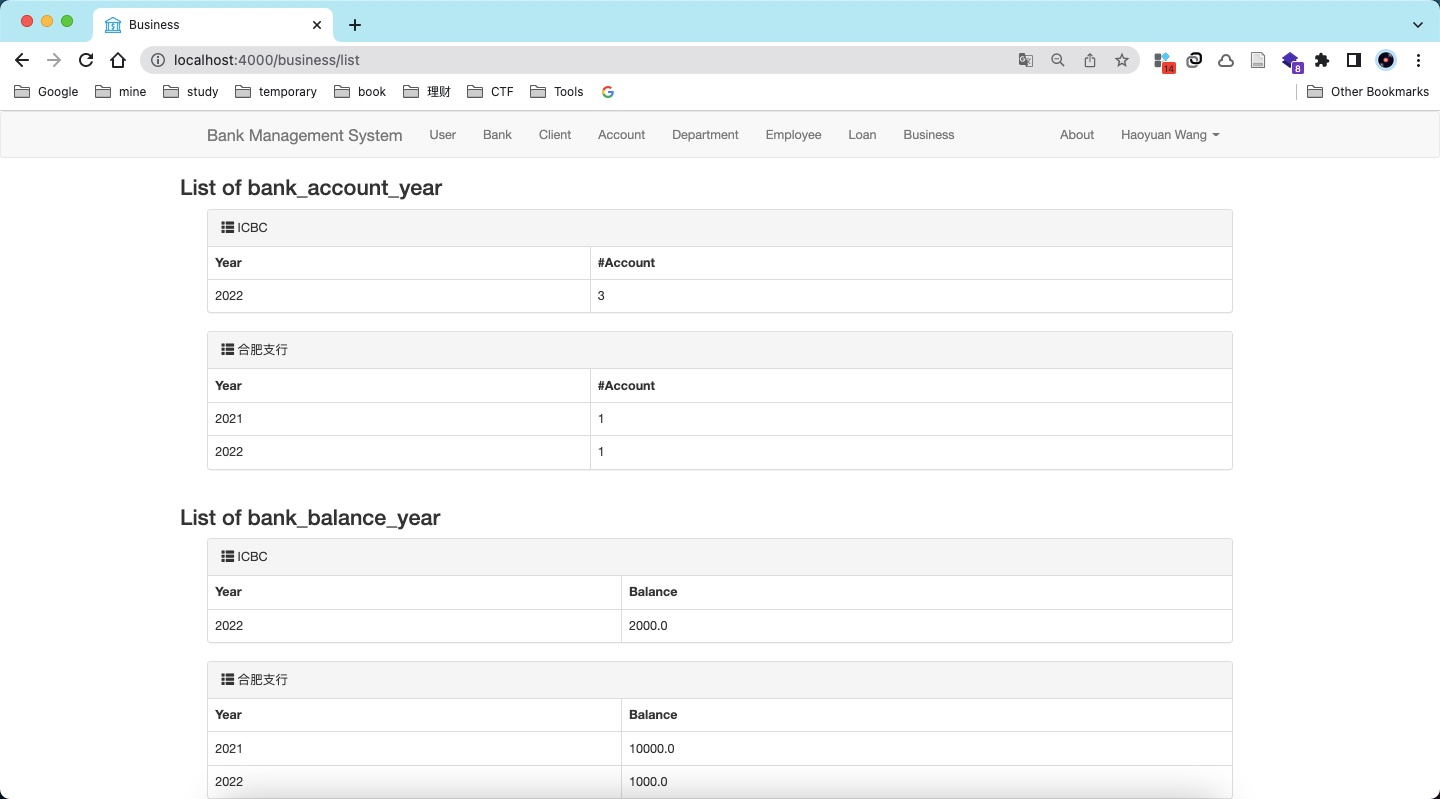
\includegraphics[width=0.8\textwidth]{./fig/business_list.jpg}
        \caption[business_list]{业务统计(因页面太长不太完整)}
    \end{figure}
    \subsection{测试结果}
    \begin{figure}[H]
        \centering
        \subfigure[之前]{
            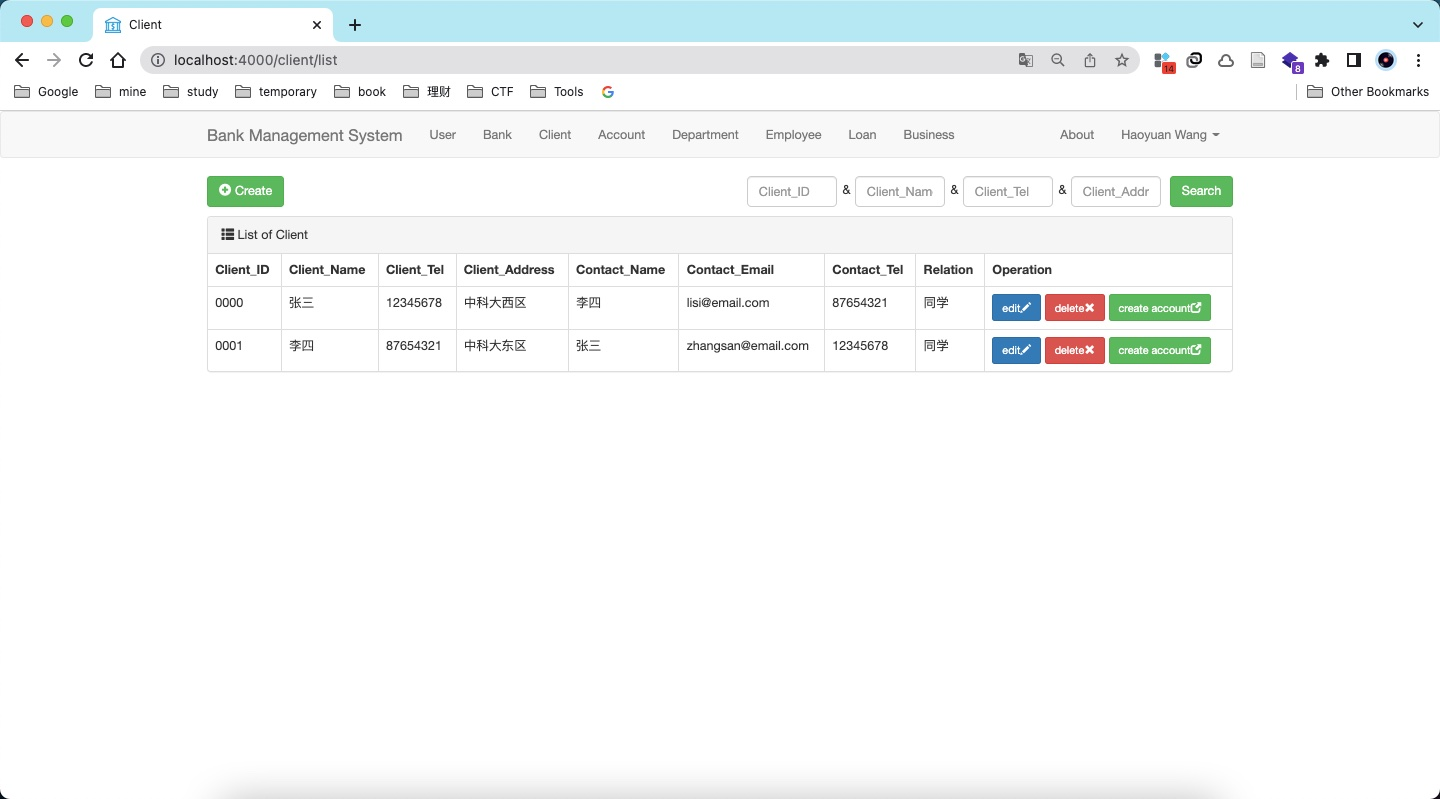
\includegraphics[width=0.4\textwidth]{./fig/client_list.jpg}
        }
        \subfigure[之后]{
            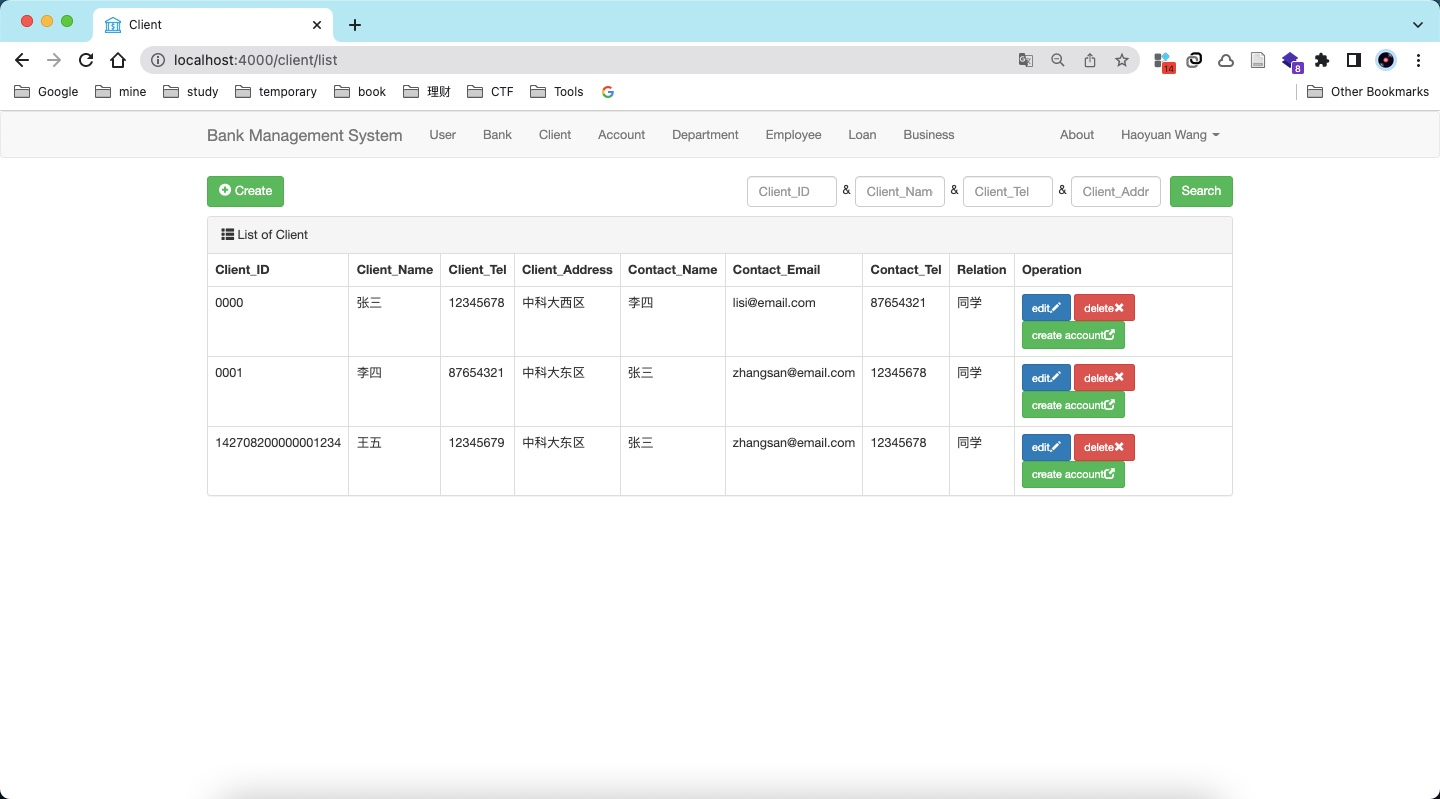
\includegraphics[width=0.4\textwidth]{./fig/add_client.jpg}
        }
        \caption{增加客户}
    \end{figure}
    \begin{figure}[H]
        \centering
        \subfigure[之前]{
            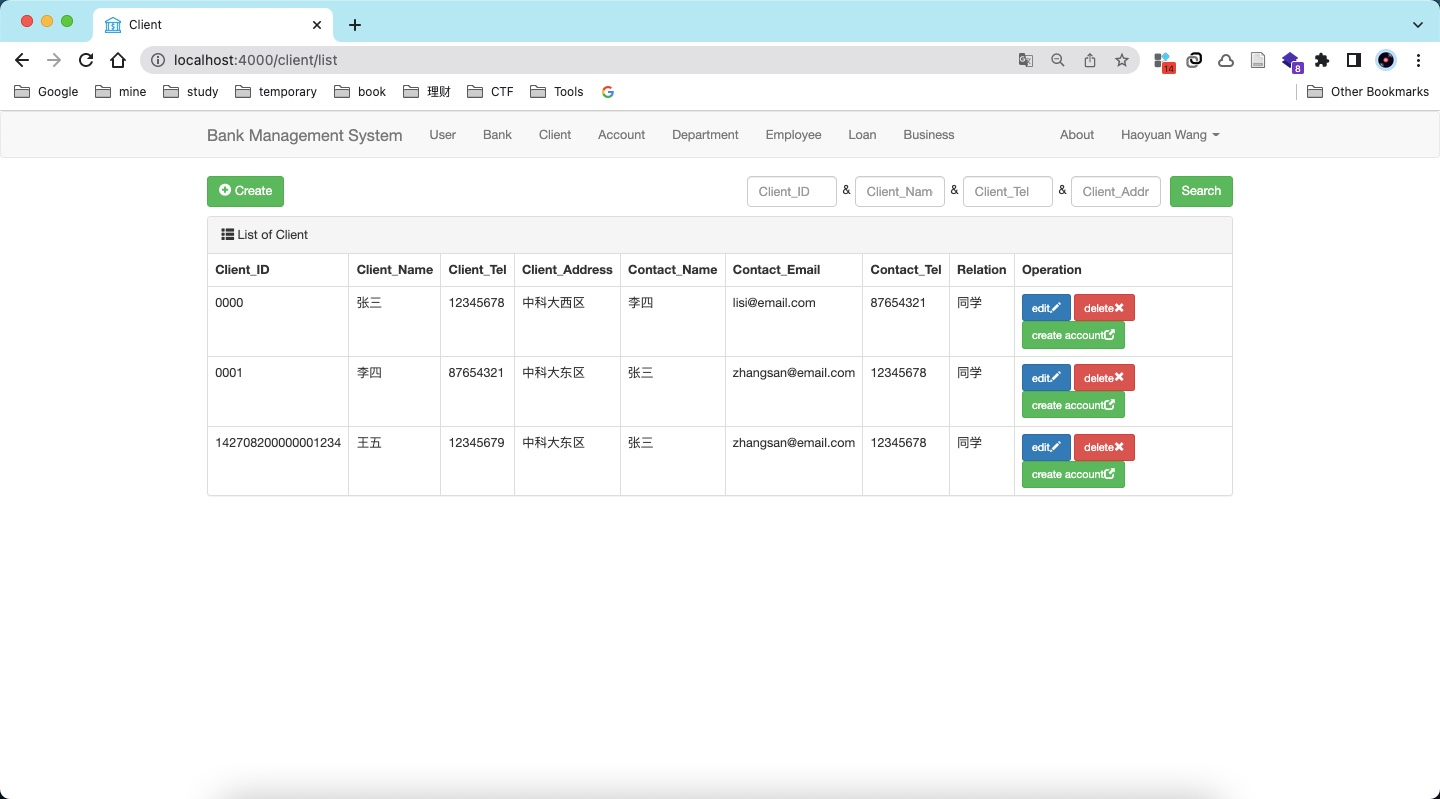
\includegraphics[width=0.4\textwidth]{./fig/add_client.jpg}
        }
        \subfigure[之后]{
            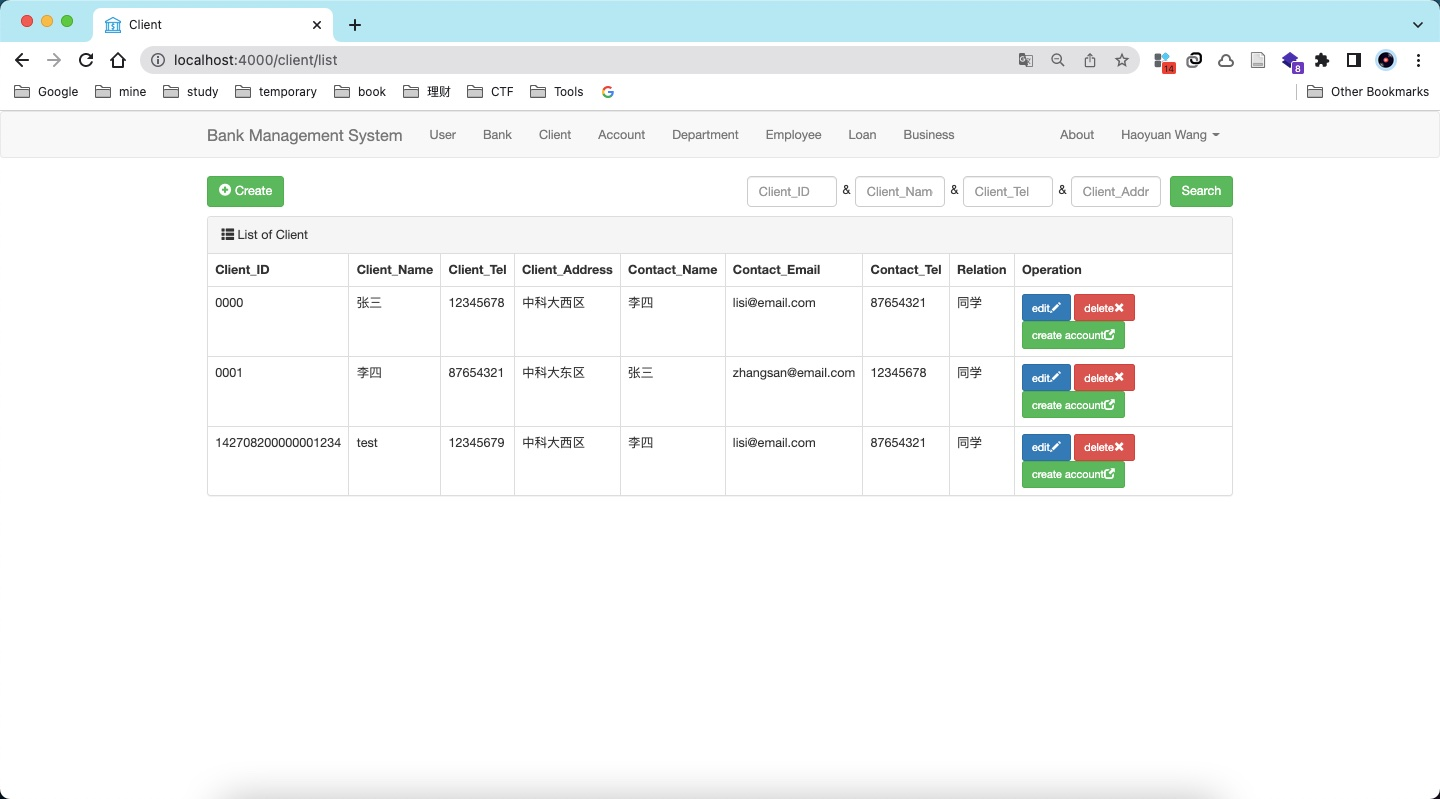
\includegraphics[width=0.4\textwidth]{./fig/edit_client.jpg}
        }
        \caption{修改客户信息}
    \end{figure}
    \begin{figure}[H]
        \centering
        \subfigure[之前]{
            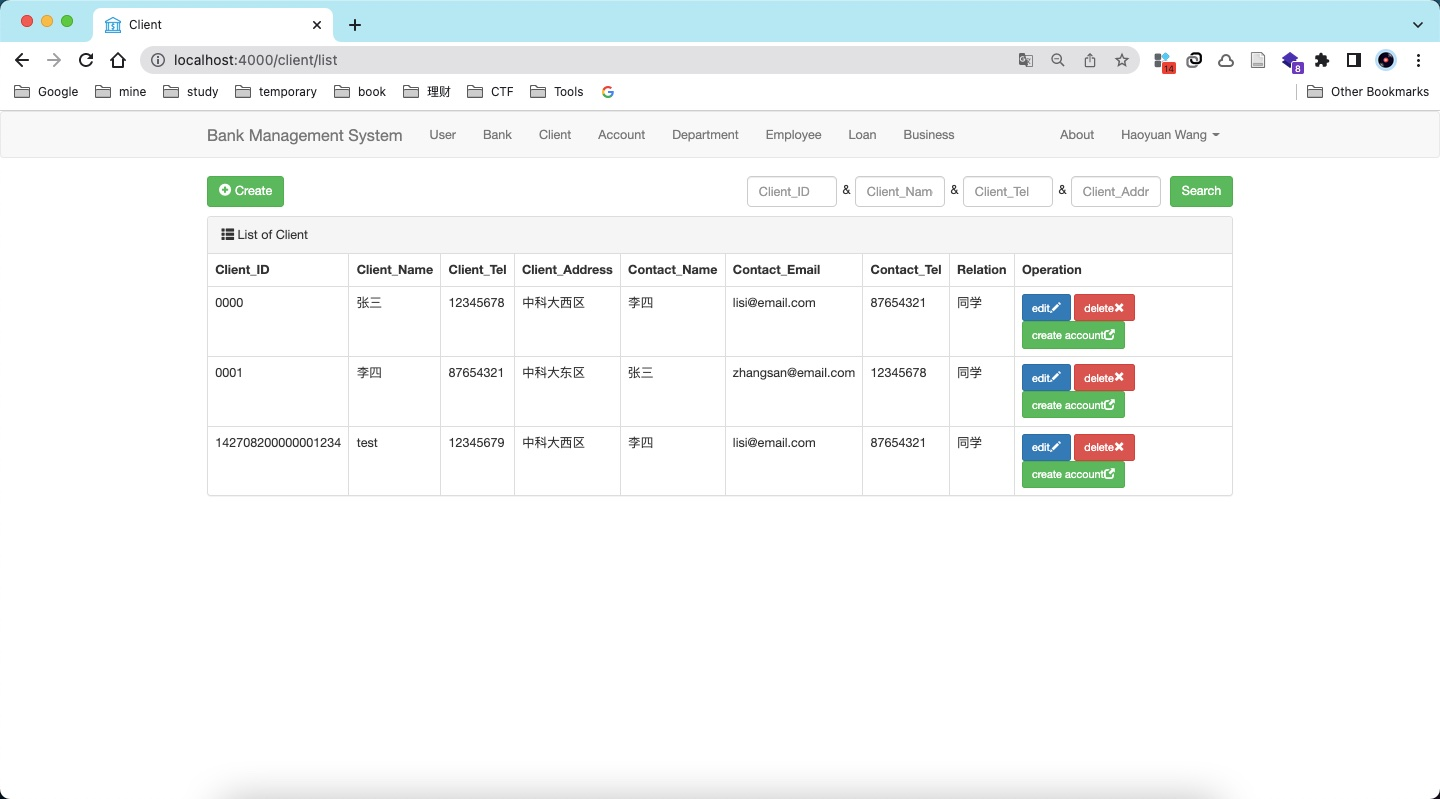
\includegraphics[width=0.4\textwidth]{./fig/edit_client.jpg}
        }
        \subfigure[之后]{
            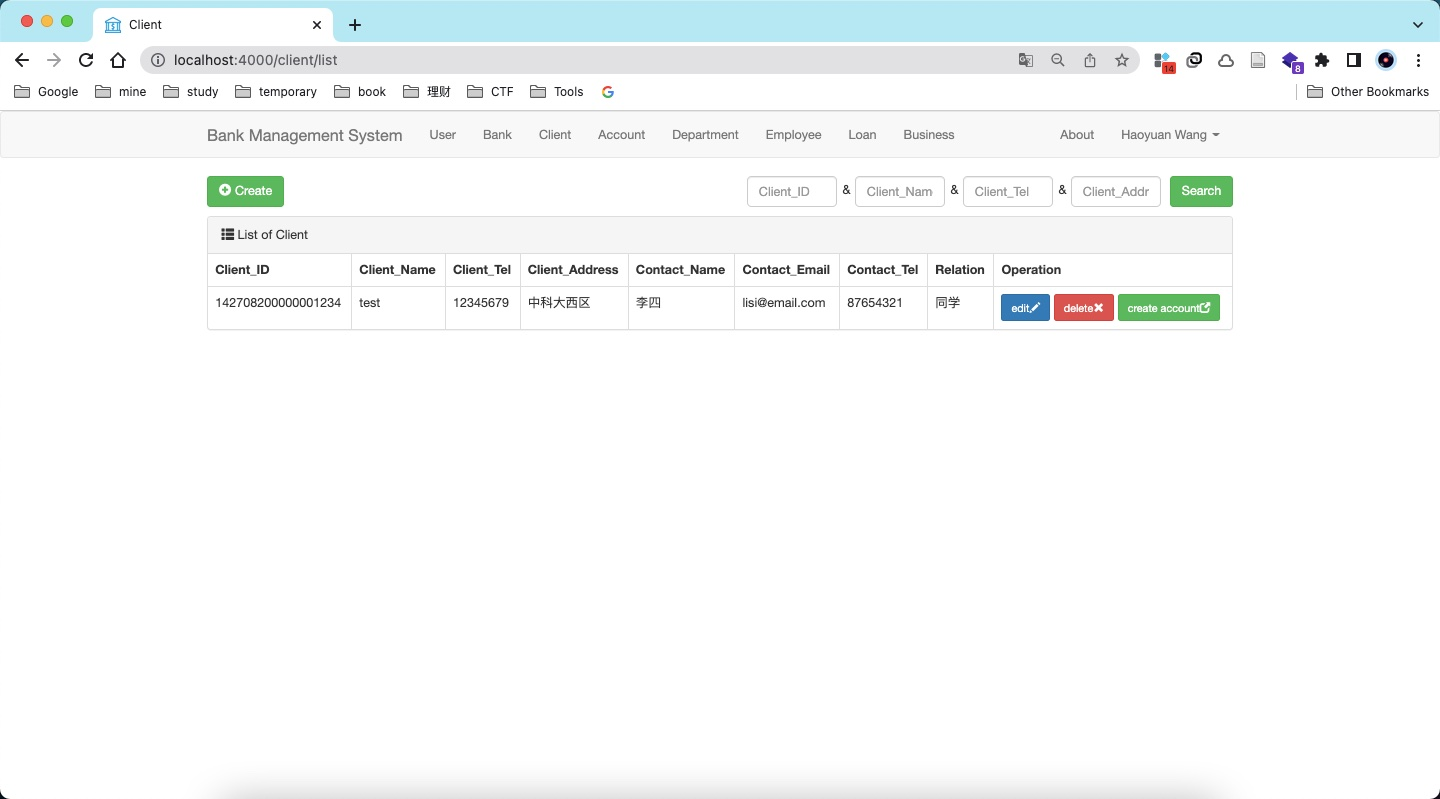
\includegraphics[width=0.4\textwidth]{./fig/client_search.jpg}
        }
        \caption{客户查询}
    \end{figure}
    \begin{figure}[H]
        \centering
        \subfigure[之前]{
            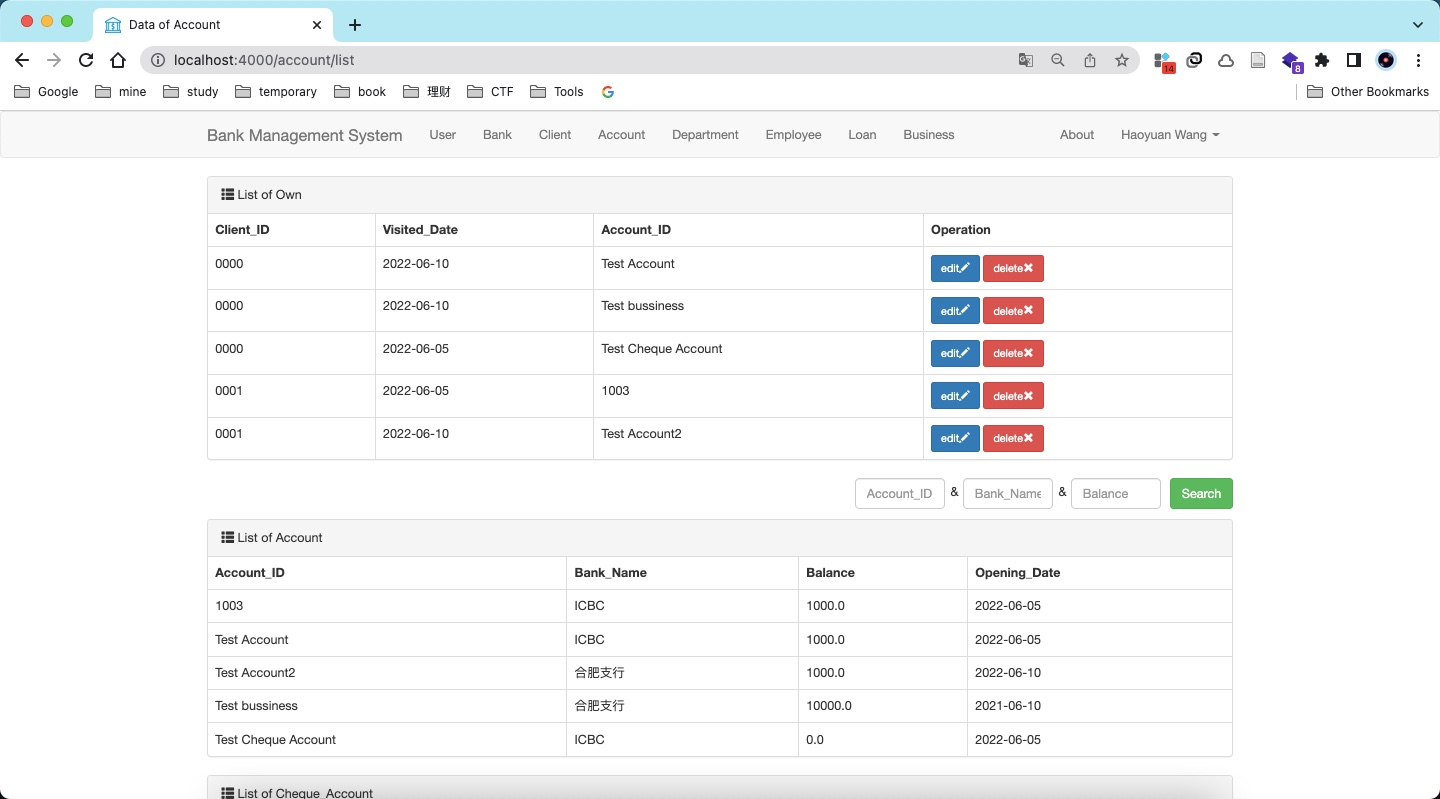
\includegraphics[width=0.4\textwidth]{./fig/account_list.jpg}
        }
        \subfigure[之后]{
            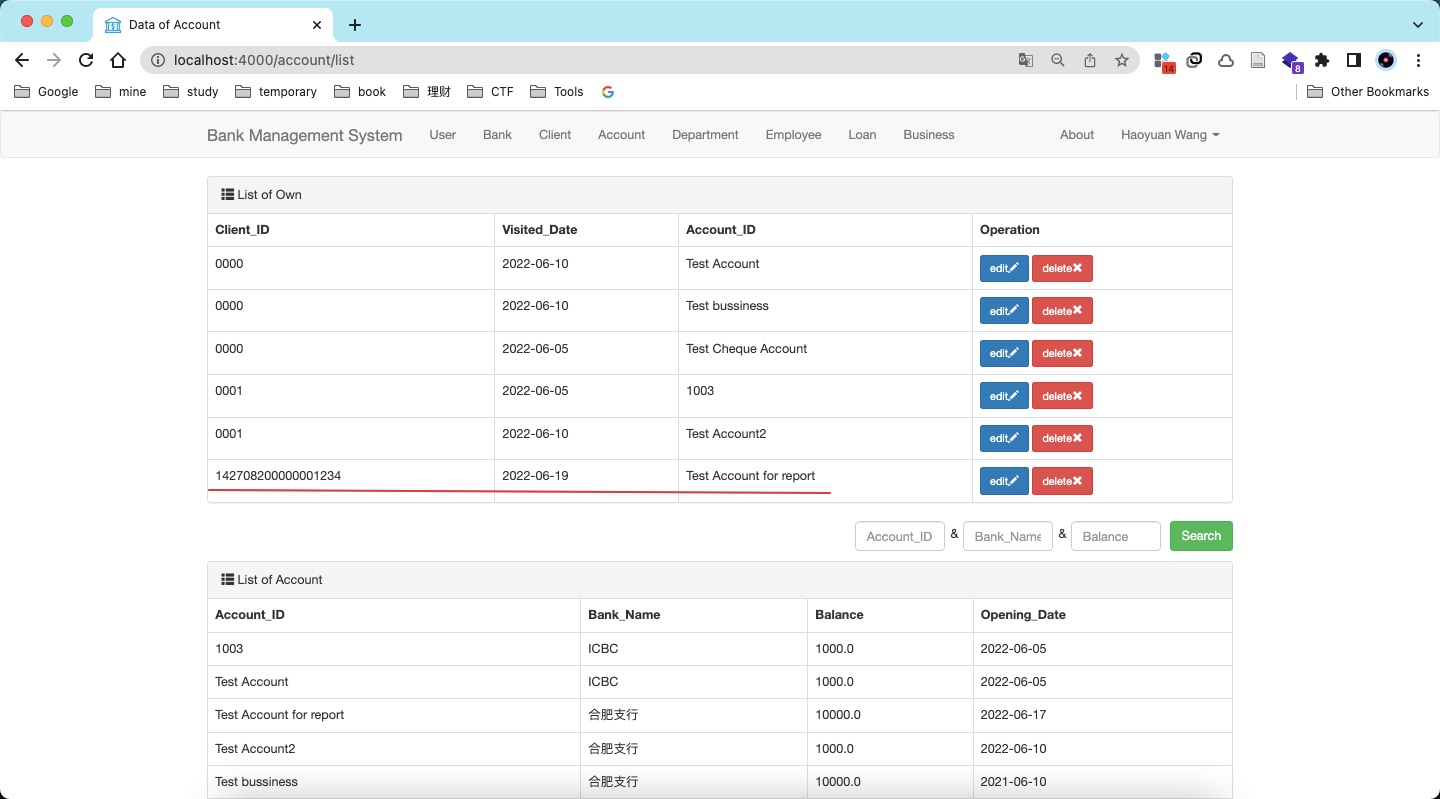
\includegraphics[width=0.4\textwidth]{./fig/create_account.jpg}
        }
        \caption{账户开户}
    \end{figure}
    \begin{figure}[H]
        \centering
        \subfigure[之前]{
            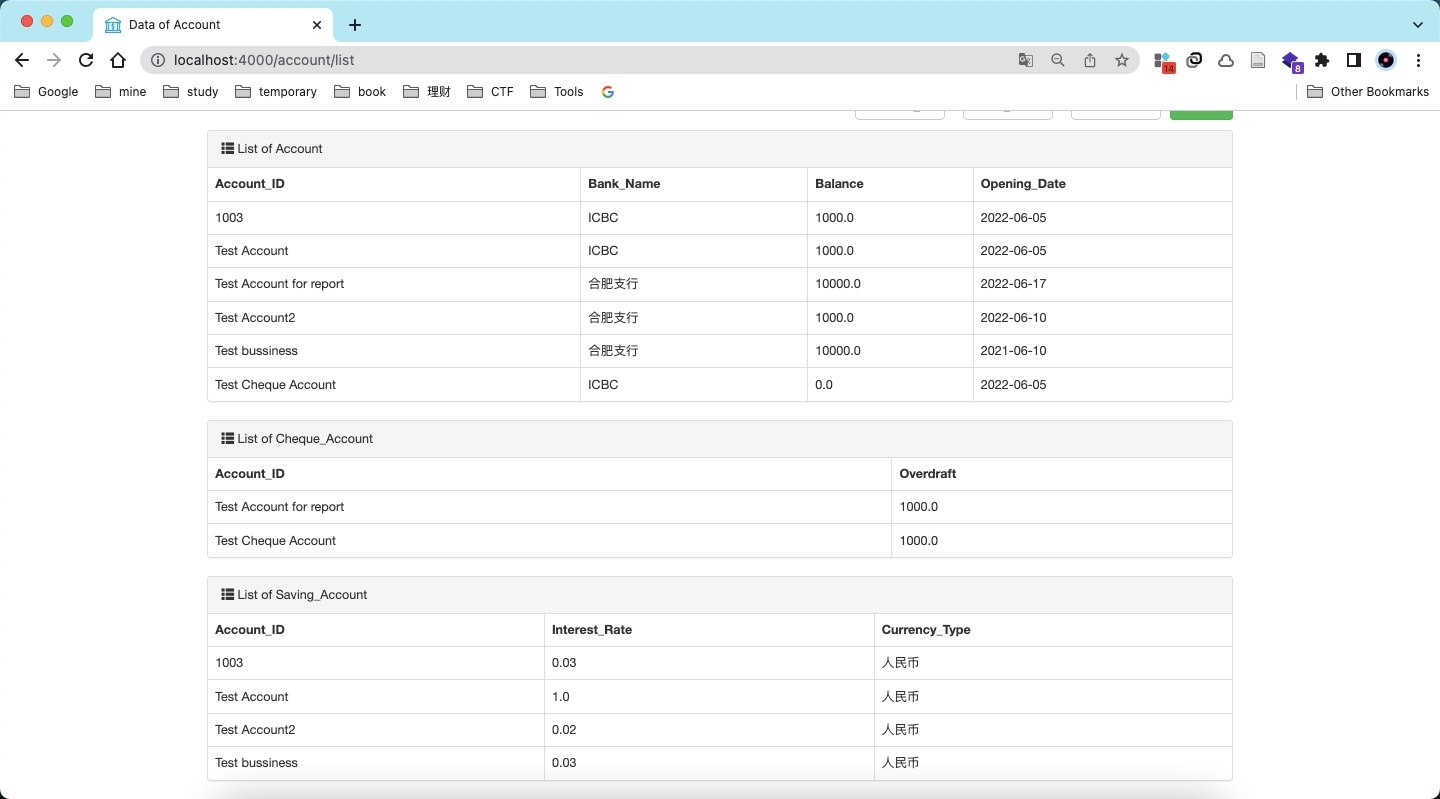
\includegraphics[width=0.4\textwidth]{./fig/account_before_edit.jpg}
        }
        \subfigure[之后]{
            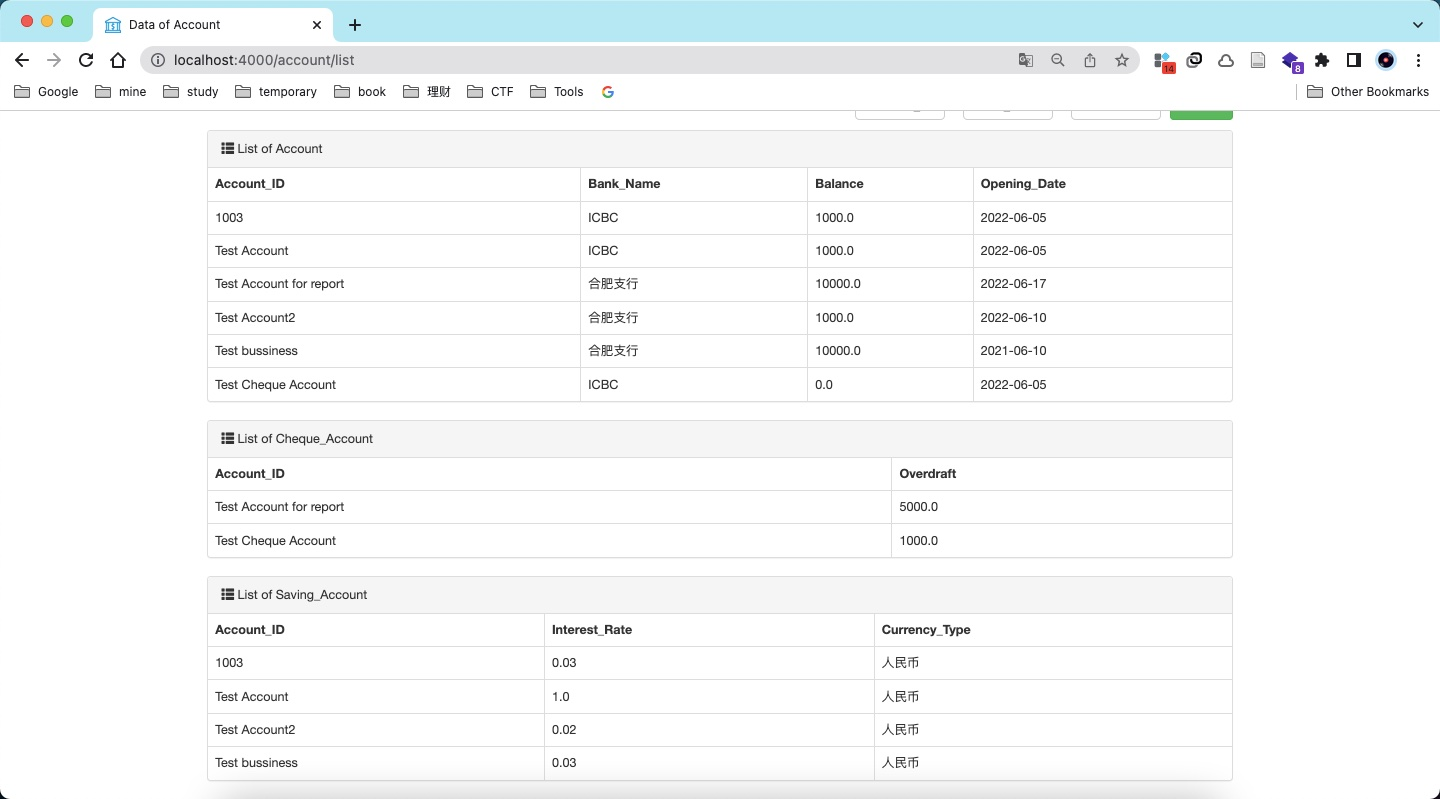
\includegraphics[width=0.4\textwidth]{./fig/account_after_edit.jpg}
        }
        \caption{修改账户信息}
    \end{figure}
    \begin{figure}[H]
        \centering
        \subfigure[之前]{
            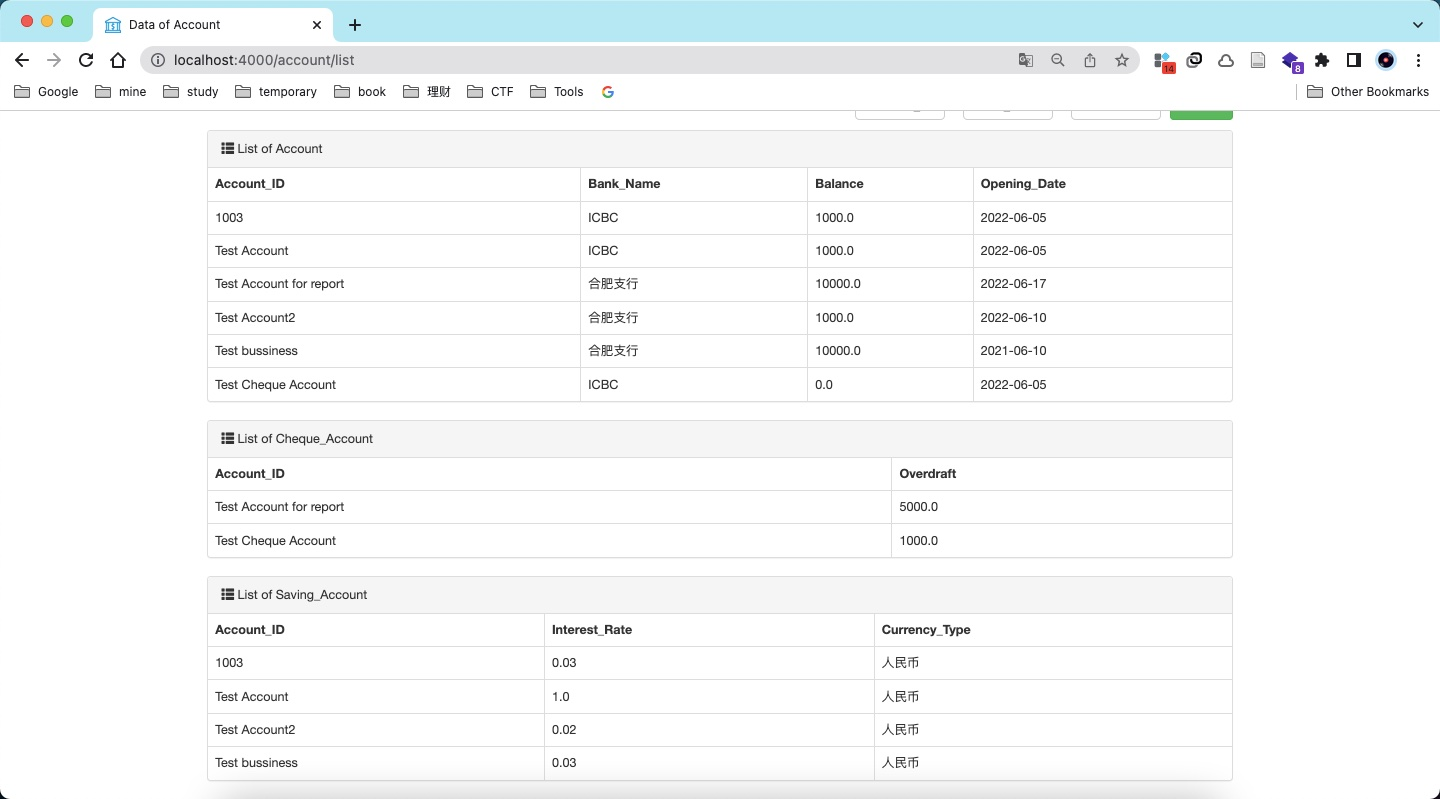
\includegraphics[width=0.4\textwidth]{./fig/account_after_edit.jpg}
        }
        \subfigure[之后]{
            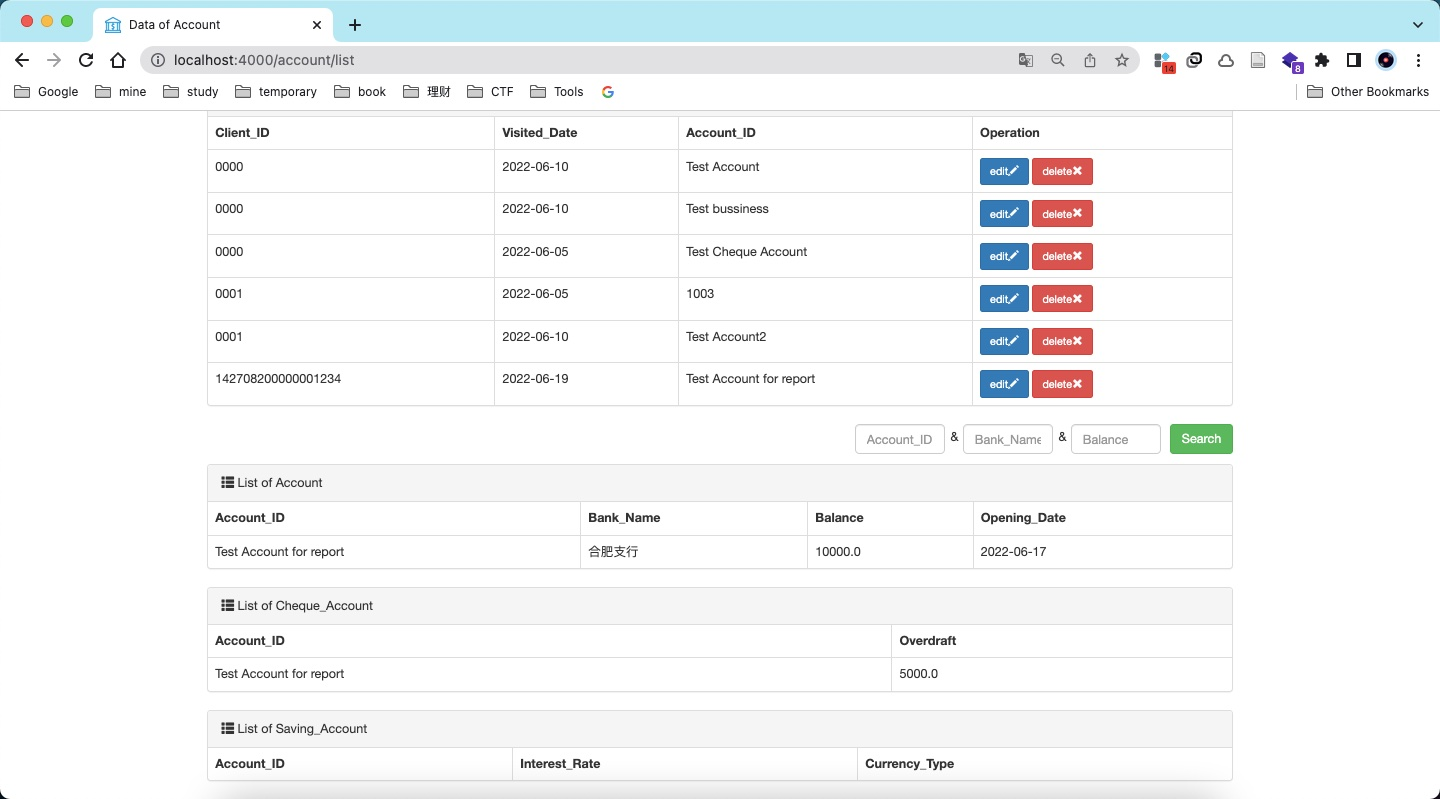
\includegraphics[width=0.4\textwidth]{./fig/account_search.jpg}
        }
        \caption{查询账户}
    \end{figure}
    \begin{figure}[H]
        \centering
        \subfigure[之前]{
            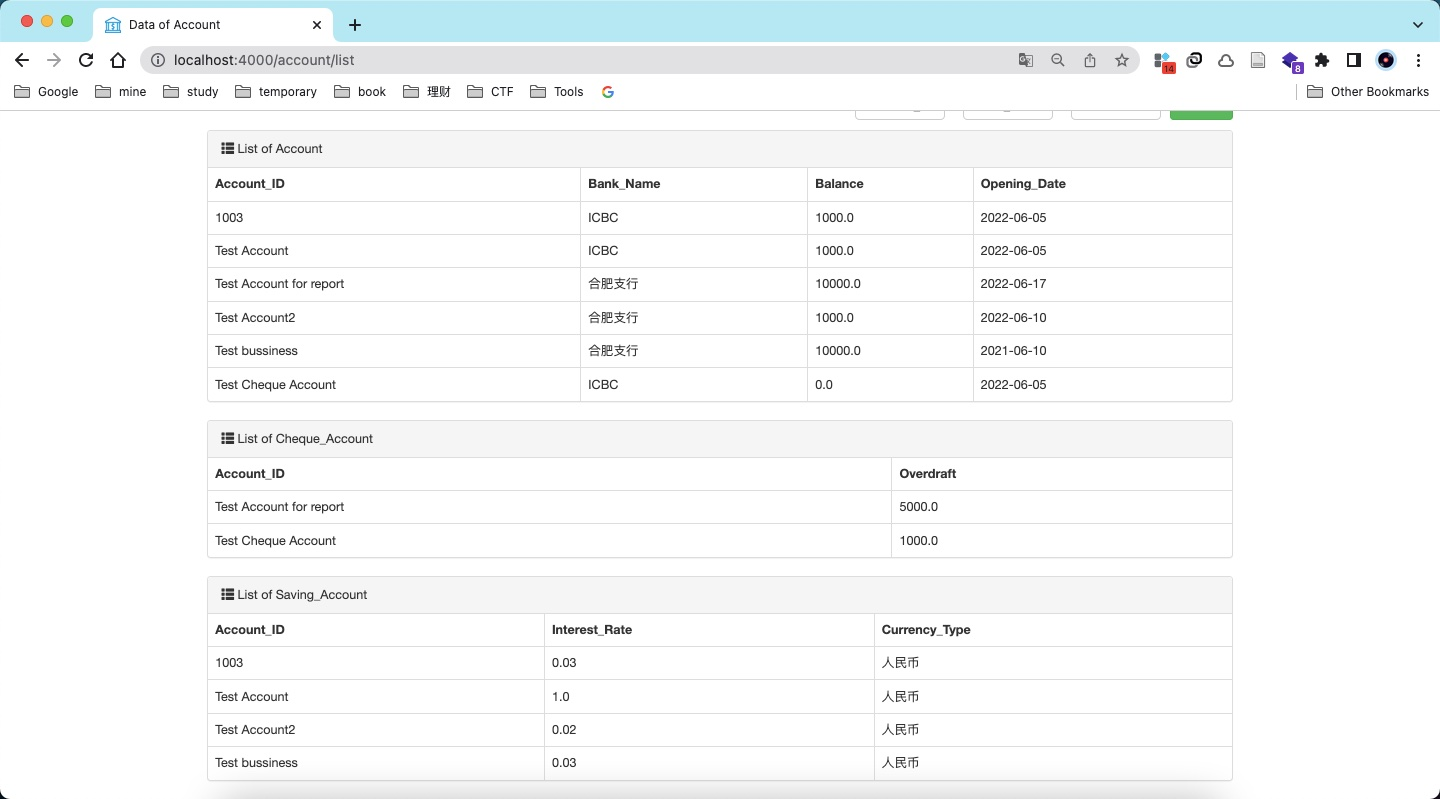
\includegraphics[width=0.4\textwidth]{./fig/account_after_edit.jpg}
        }
        \subfigure[之后]{
            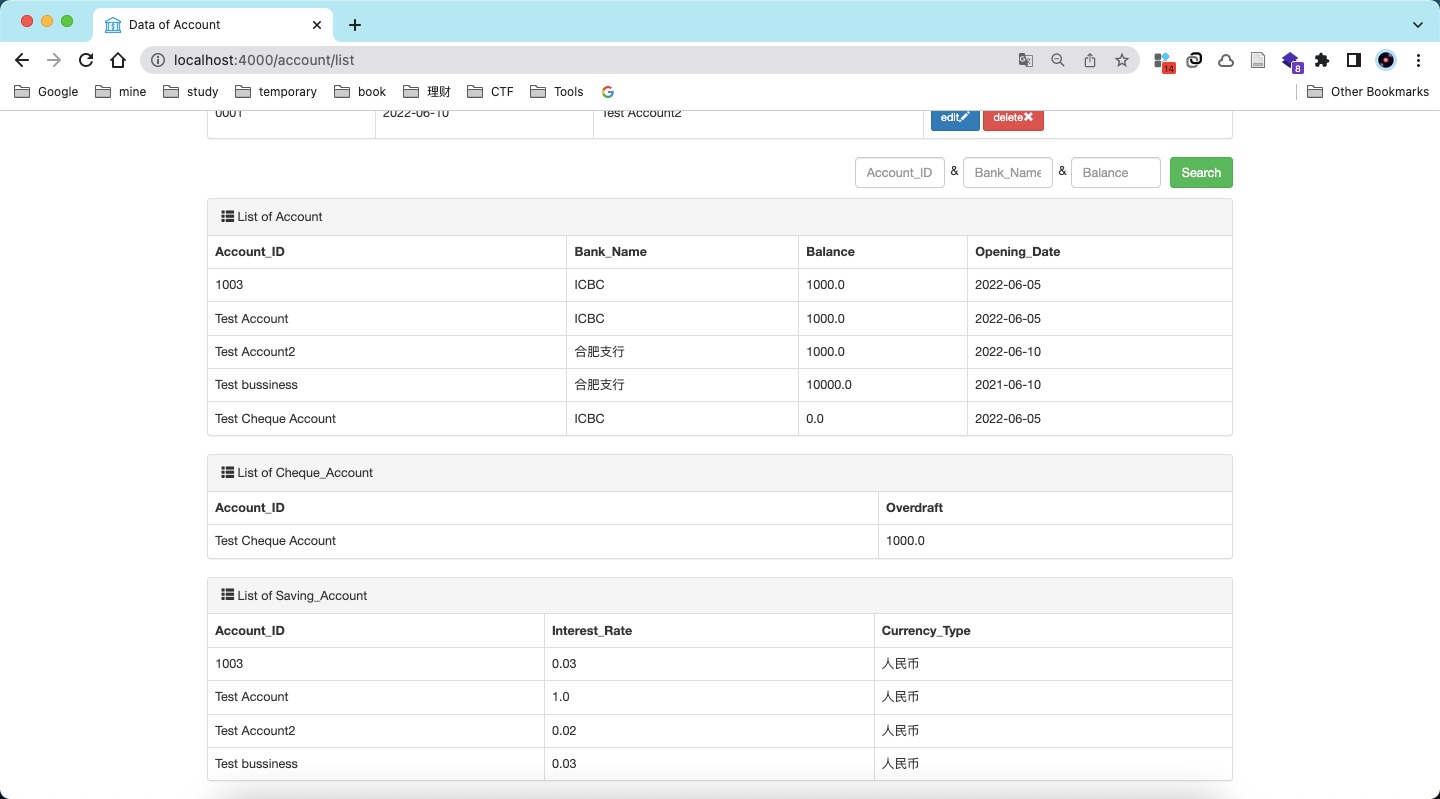
\includegraphics[width=0.4\textwidth]{./fig/account_after_delete.jpg}
        }
        \caption{账户销户}
    \end{figure}
    \begin{figure}[H]
        \centering
        \subfigure[之前]{
            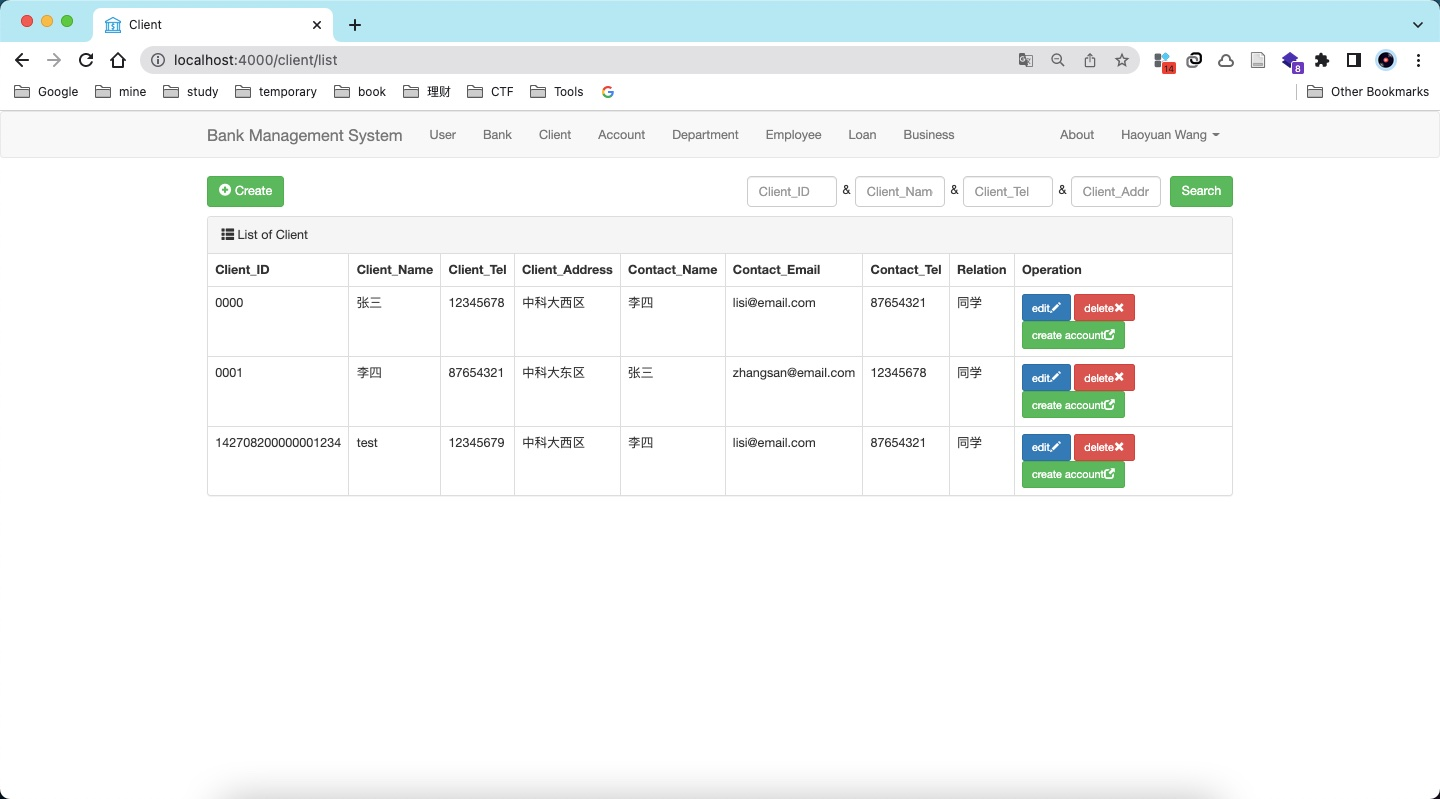
\includegraphics[width=0.4\textwidth]{./fig/edit_client.jpg}
        }
        \subfigure[之后]{
            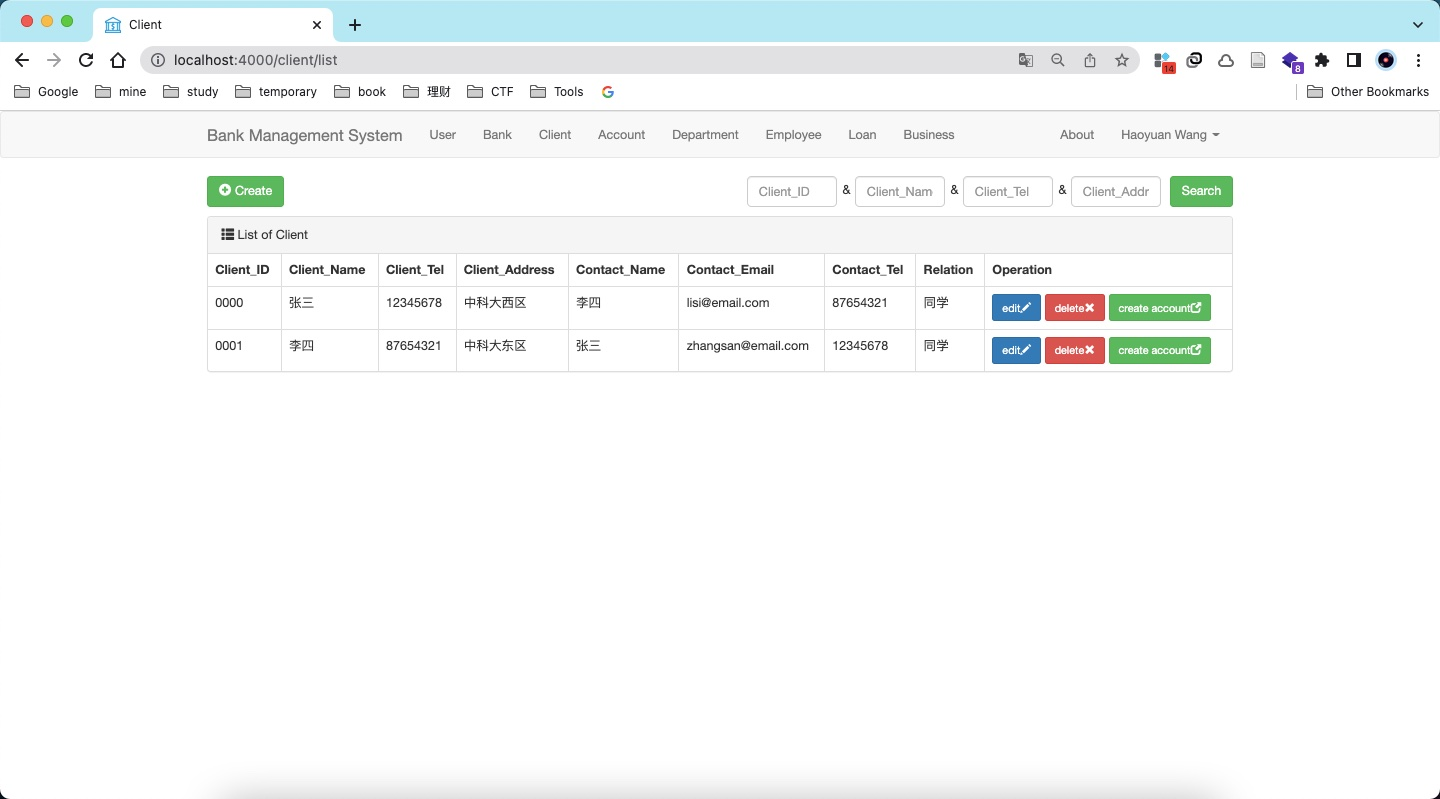
\includegraphics[width=0.4\textwidth]{./fig/client_after_delete.jpg}
        }
        \caption{删除客户}
    \end{figure}
    \begin{figure}[H]
        \centering
        \subfigure[之前]{
            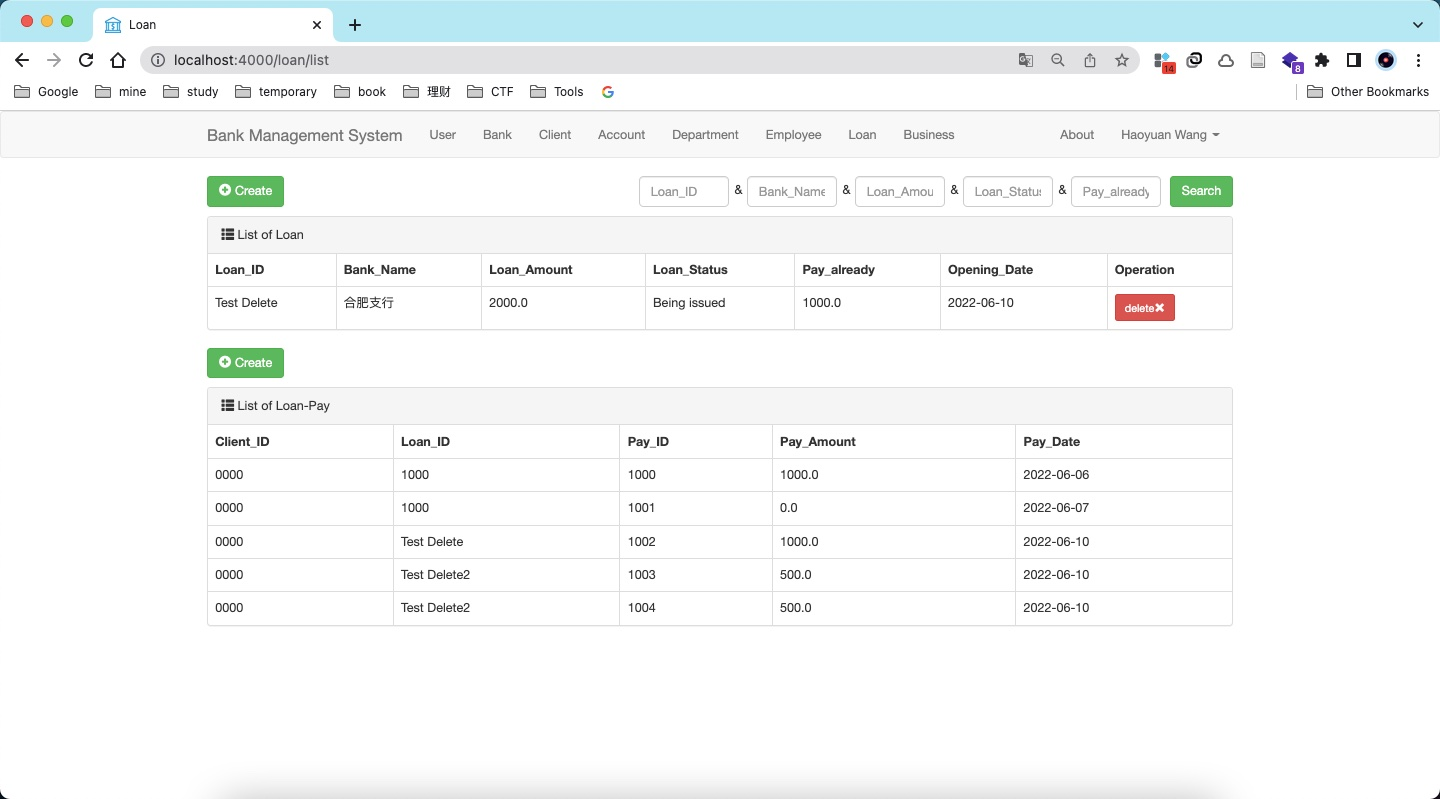
\includegraphics[width=0.4\textwidth]{./fig/loan_list.jpg}
        }
        \subfigure[之后]{
            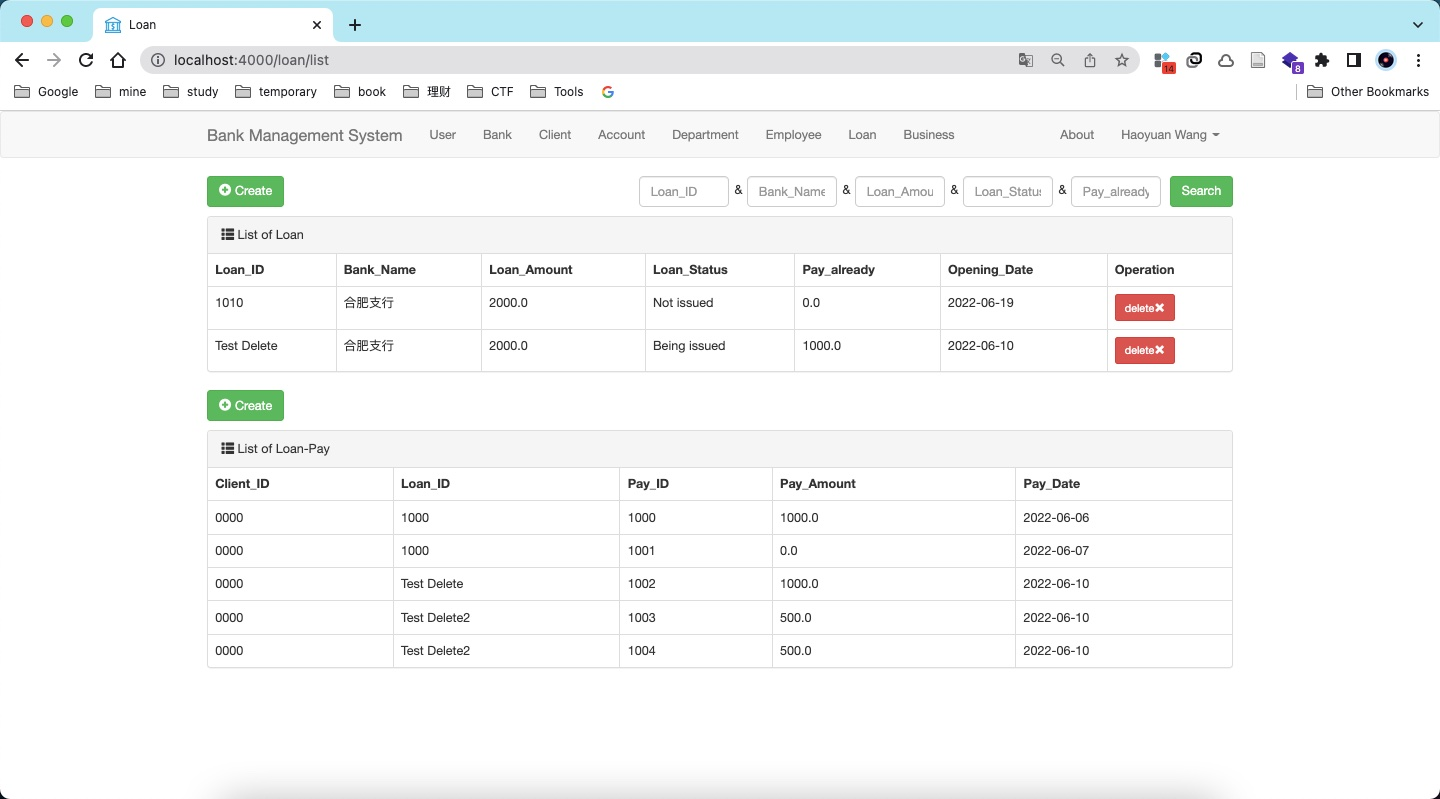
\includegraphics[width=0.4\textwidth]{./fig/add_loan.jpg}
        }
        \caption{添加贷款}
    \end{figure}
    \begin{figure}[H]
        \centering
        \subfigure[之前]{
            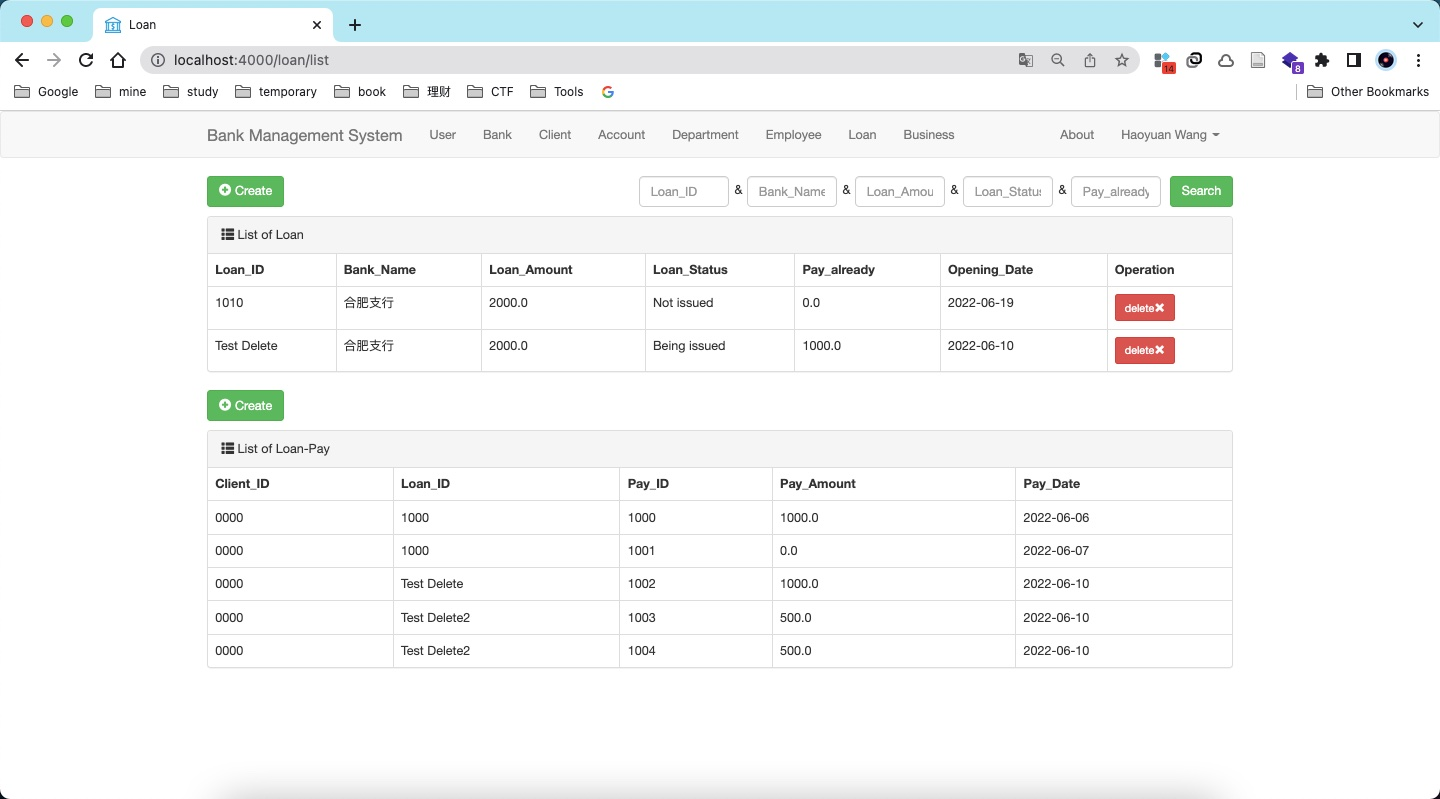
\includegraphics[width=0.4\textwidth]{./fig/add_loan.jpg}
        }
        \subfigure[之后]{
            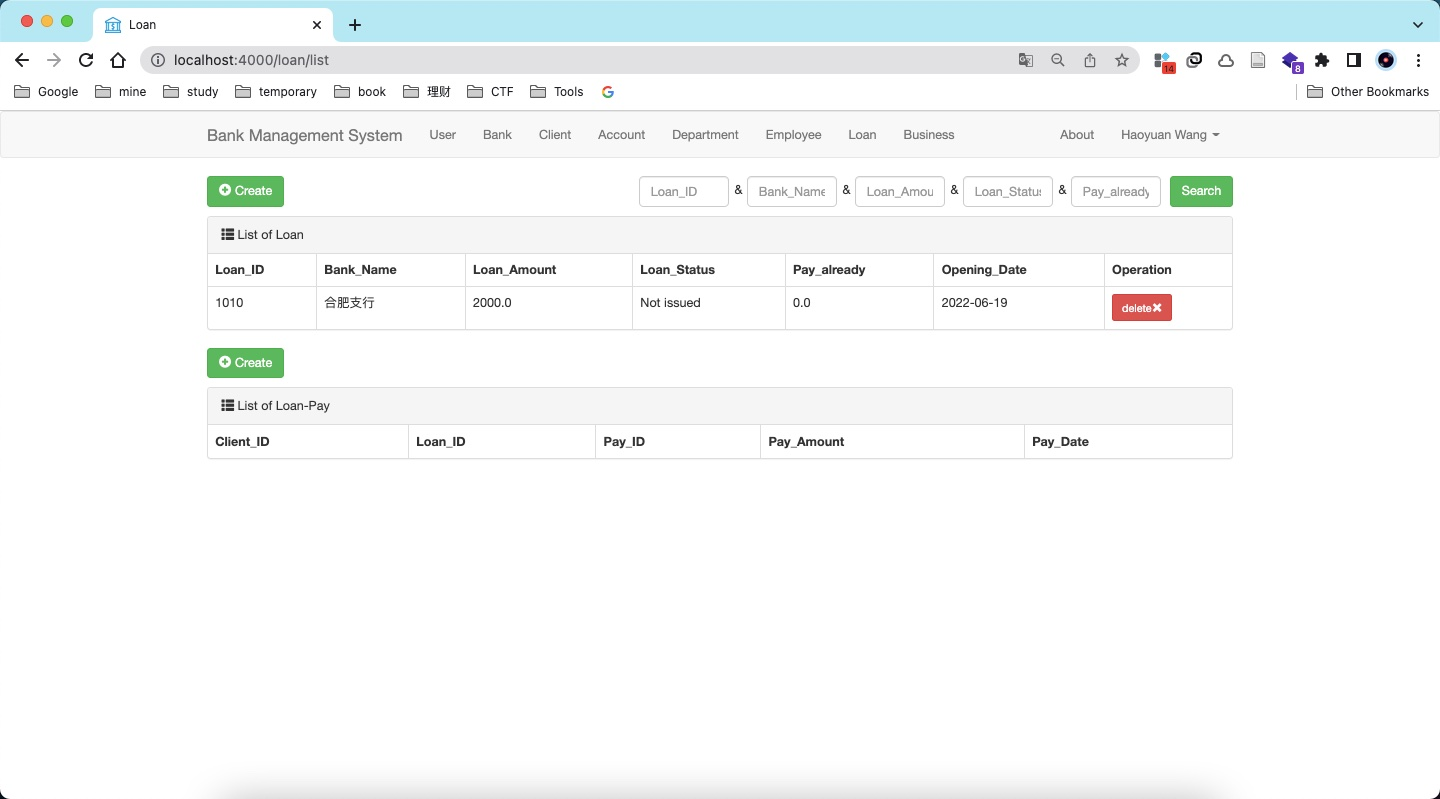
\includegraphics[width=0.4\textwidth]{./fig/loan_search.jpg}
        }
        \caption{贷款查询}
    \end{figure}
    \begin{figure}[H]
        \centering
        \subfigure[未发放贷款]{
            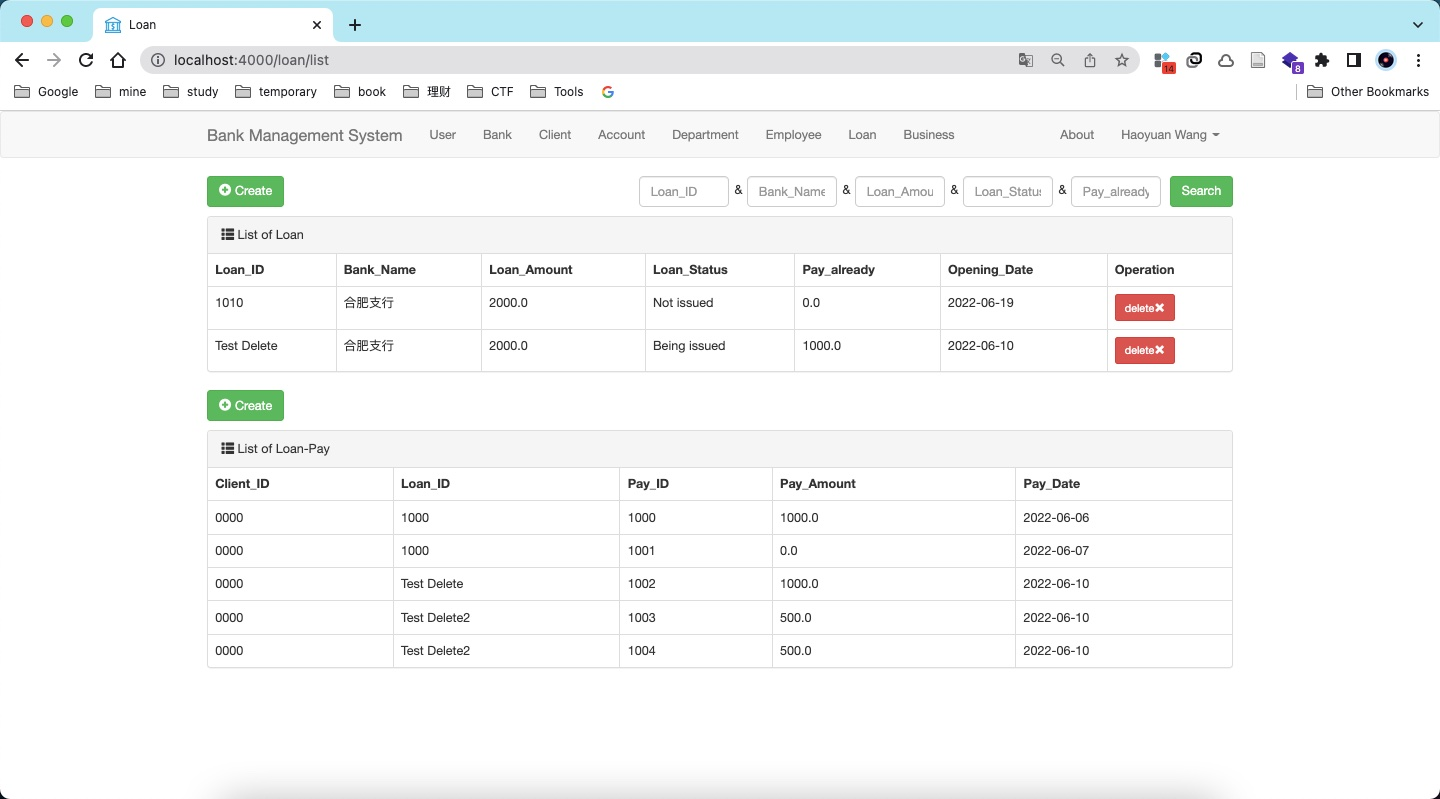
\includegraphics[width=0.3\textwidth]{./fig/add_loan.jpg}
        }
        \subfigure[发放部分贷款]{
            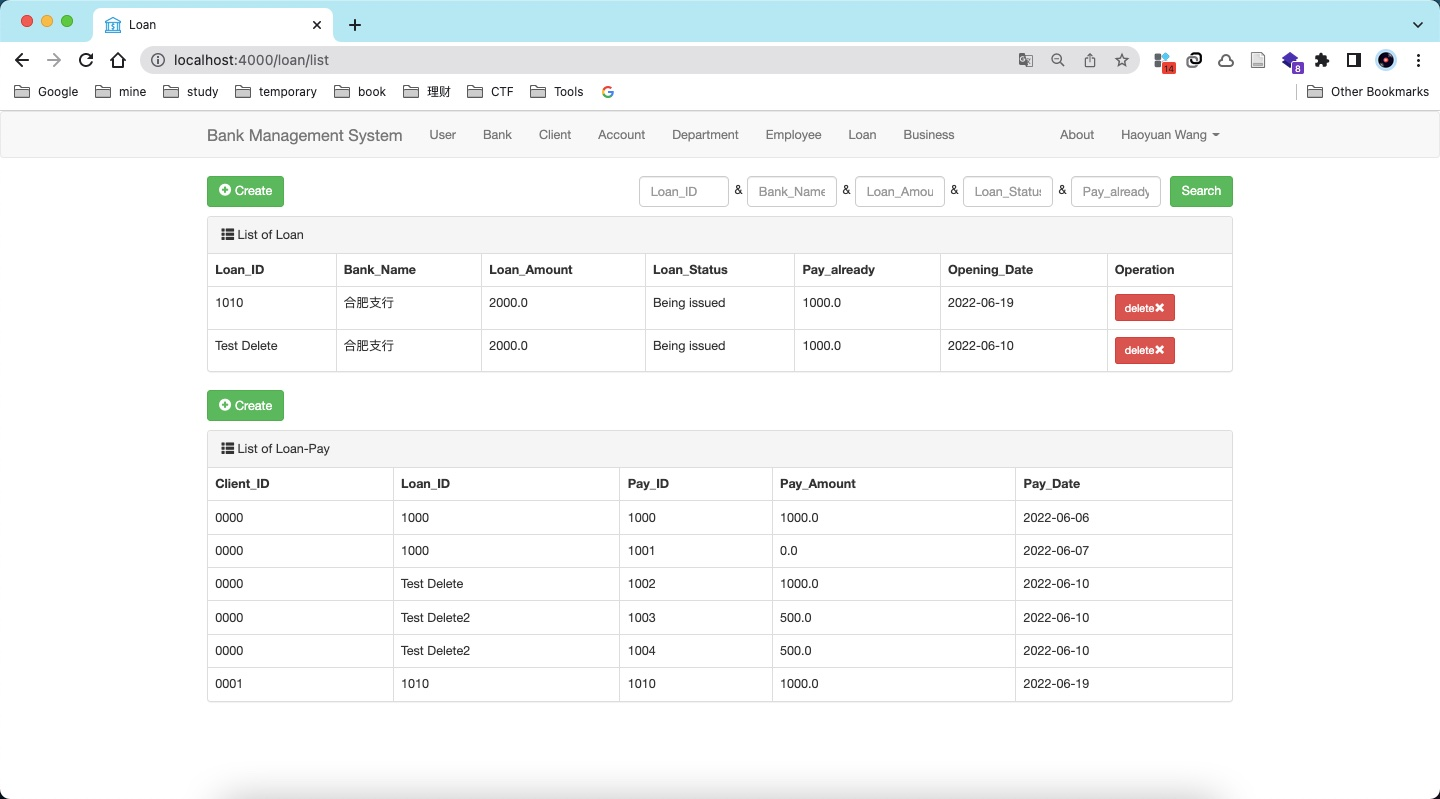
\includegraphics[width=0.3\textwidth]{./fig/pay_part_loan.jpg}
        }
        \subfigure[发放所有贷款]{
            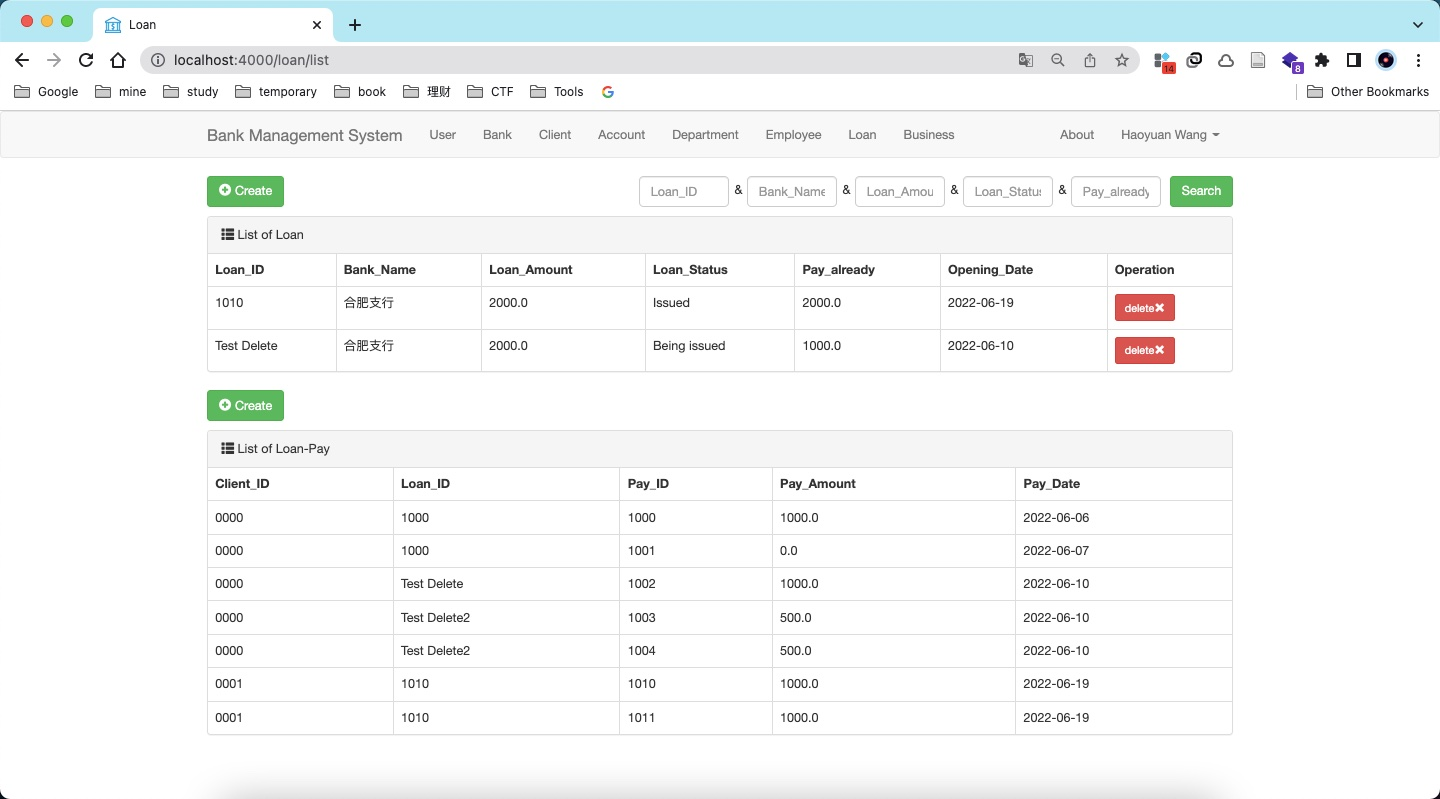
\includegraphics[width=0.3\textwidth]{./fig/pay_all_loan.jpg}
        }
        \caption{贷款发放}
    \end{figure}
    \begin{figure}[H]
        \centering
        \subfigure[之前]{
            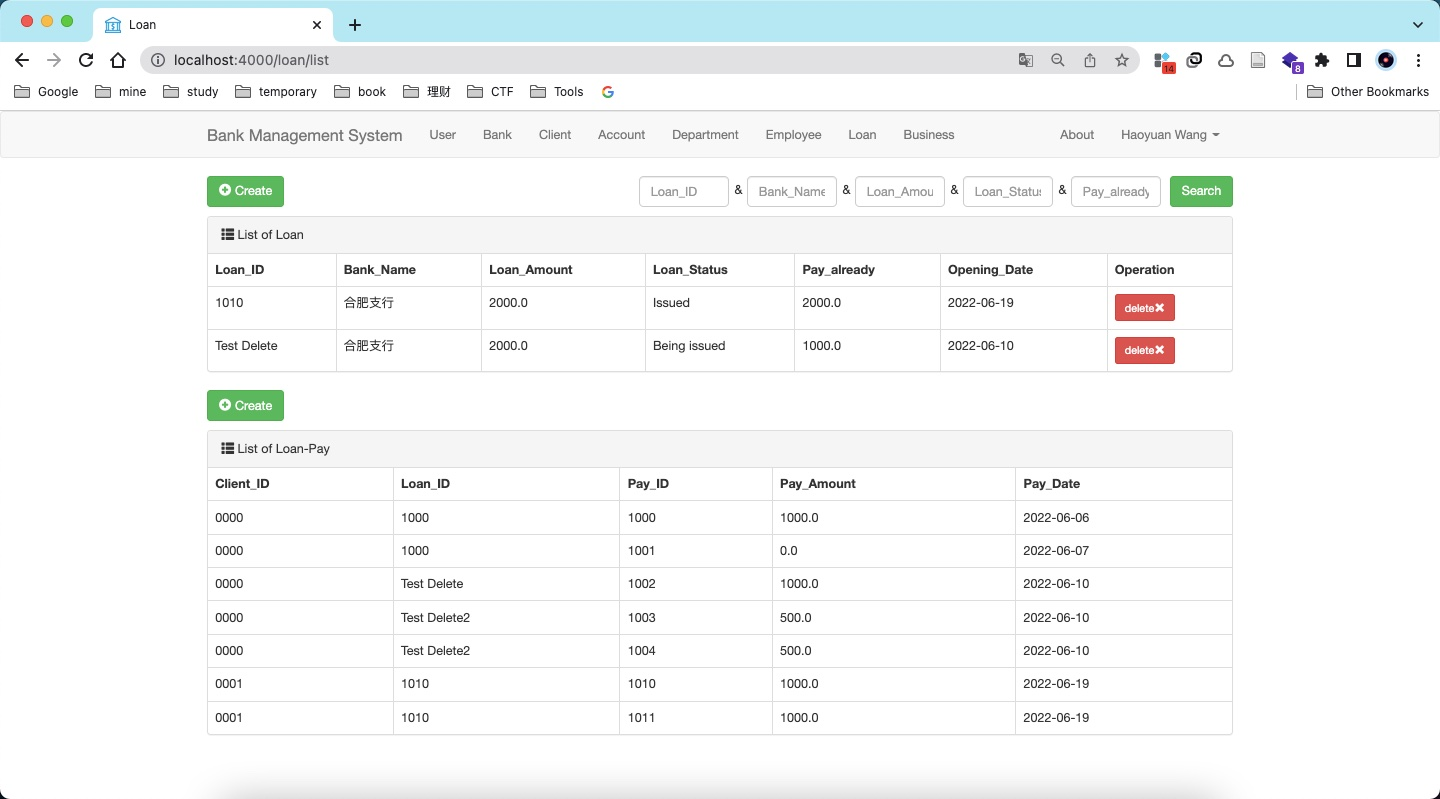
\includegraphics[width=0.4\textwidth]{./fig/pay_all_loan.jpg}
        }
        \subfigure[之后]{
            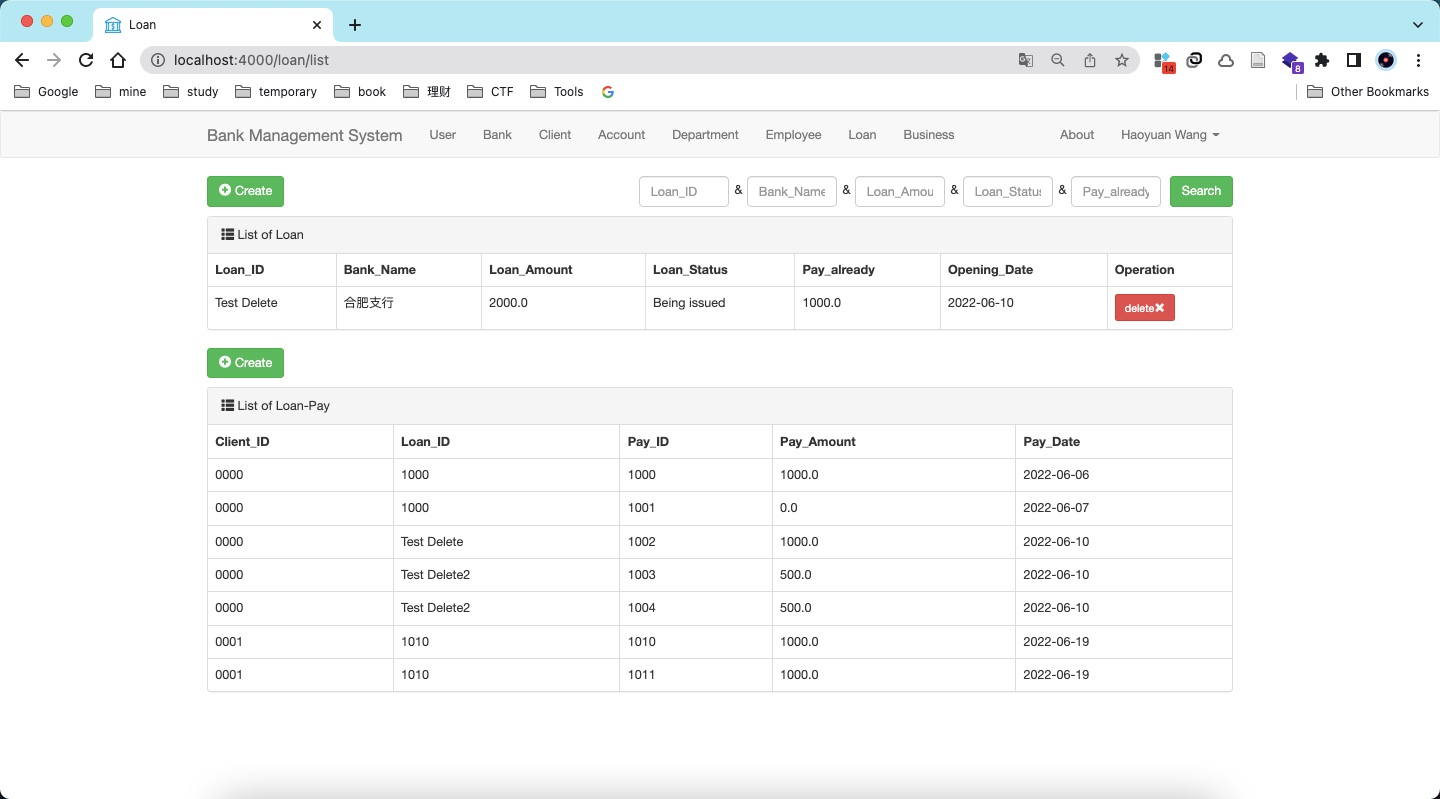
\includegraphics[width=0.4\textwidth]{./fig/delete_loan.jpg}
        }
        \caption{删除贷款}
    \end{figure}
    \subsection{实现中的难点问题及解决}
    \begin{itemize}
        \item 不熟悉浏览器网页开发:主要使用w3school平台进行资料搜集和相关知识学习,
        同时向有相关经验的同学请教
        \item 前端不能正常渲染:经过检查和测试,会发现某些时候是自己布局写的有问题,而某些时候可能因为cdn服务不稳定导致(可以通过下载到本地解决)
        \item 在测试时功能异常:使用Python的logging包,在关键节点处记录log,使用log进行debug
        \item 总结的常见异常情况:
        \begin{itemize}
            \item 前后端数据交互不正确(双向均有可能)
            \item MySQL语句生成错误(例如字段忘记加单引号)
            \item 没有注意由于外键约束导致的特定语句执行顺序
        \end{itemize}
        \item 实现对特殊字符(例如单引号)的处理:起初通过手动处理(将单引号替换为转义字符),
        后经过调研,发现{\jetbrains pymysql}包中有相关的处理函数,改为使用包中提供的函数进行处理
    \end{itemize}
    \section{总结与讨论}
    \begin{itemize}
        \item 本次实验通过使用Python、MySQL、HTML、CSS、JavaScript等诸多语言及工具,
        实现了一个简单的B/S模型的数据库系统,结合lab2进行数据的设计,体会到了数据库设计与实现的诸多原则,
        也在一定程度上领悟了背后的思想,进一步加深了我对数据库系统的理解,也更进一步地掌握了MySQL相关的技能。
        \item 有很多地方做得不够完善,有很大的进步空间。主要是很多约束做得还不够约束,在某些特定的条件下不会被满足。
        在这个方面我还需要做出更多的努力。
        \item 在以后和数据库相关的开发中,我会尽力去多开发数据库本身的效能,而非依靠后端开发来检验数据正确性、完整性。
    \end{itemize}
    
\end{document}